\chapter{Language Overview}
\label{chap:lang-overview}

\section{Introduction}

This chapter provides the background knowledge 
to understand \pharmml. We recommend that you read this chapter
before working through the examples in chapter
\ref{chap:worked-egs}. The chapter starts by describing how a
\pharmml document is organised and then go on to illustrate some of
the key concepts and constructs of the language. For example, among
other things, we discuss variable and parameter scoping (section
\ref{sec:scoping-rules}), how to write maths (sections~\ref{sec:odes}
and~\ref{sec:maths}), and how to define data (section~\ref{subsec:inlineDataset}).
%and how to define and use units (section~\ref{sec:units}).
The chapter concludes with a discussion of the additional resources that
we expect to be used in support of \pharmml, but which are outside the
scope of this language specification (section~\ref{sec:supporting-res}).

\section{Organisation of \pharmml}
\label{sec:structure-overview}

\pharmml is organised into three main sections (\ref{fig:momloverview}): \emph{Model Definition}, \emph{Trial
  Design} and \emph{Modelling Steps}. This reflects the natural
organisation of a pharmacometric model and is the organisation
implicitly found in the M\&S tools used by modellers in this
area. Below we detail the purpose and
organisation of each section.

\begin{figure}[htb!]
 \centering
  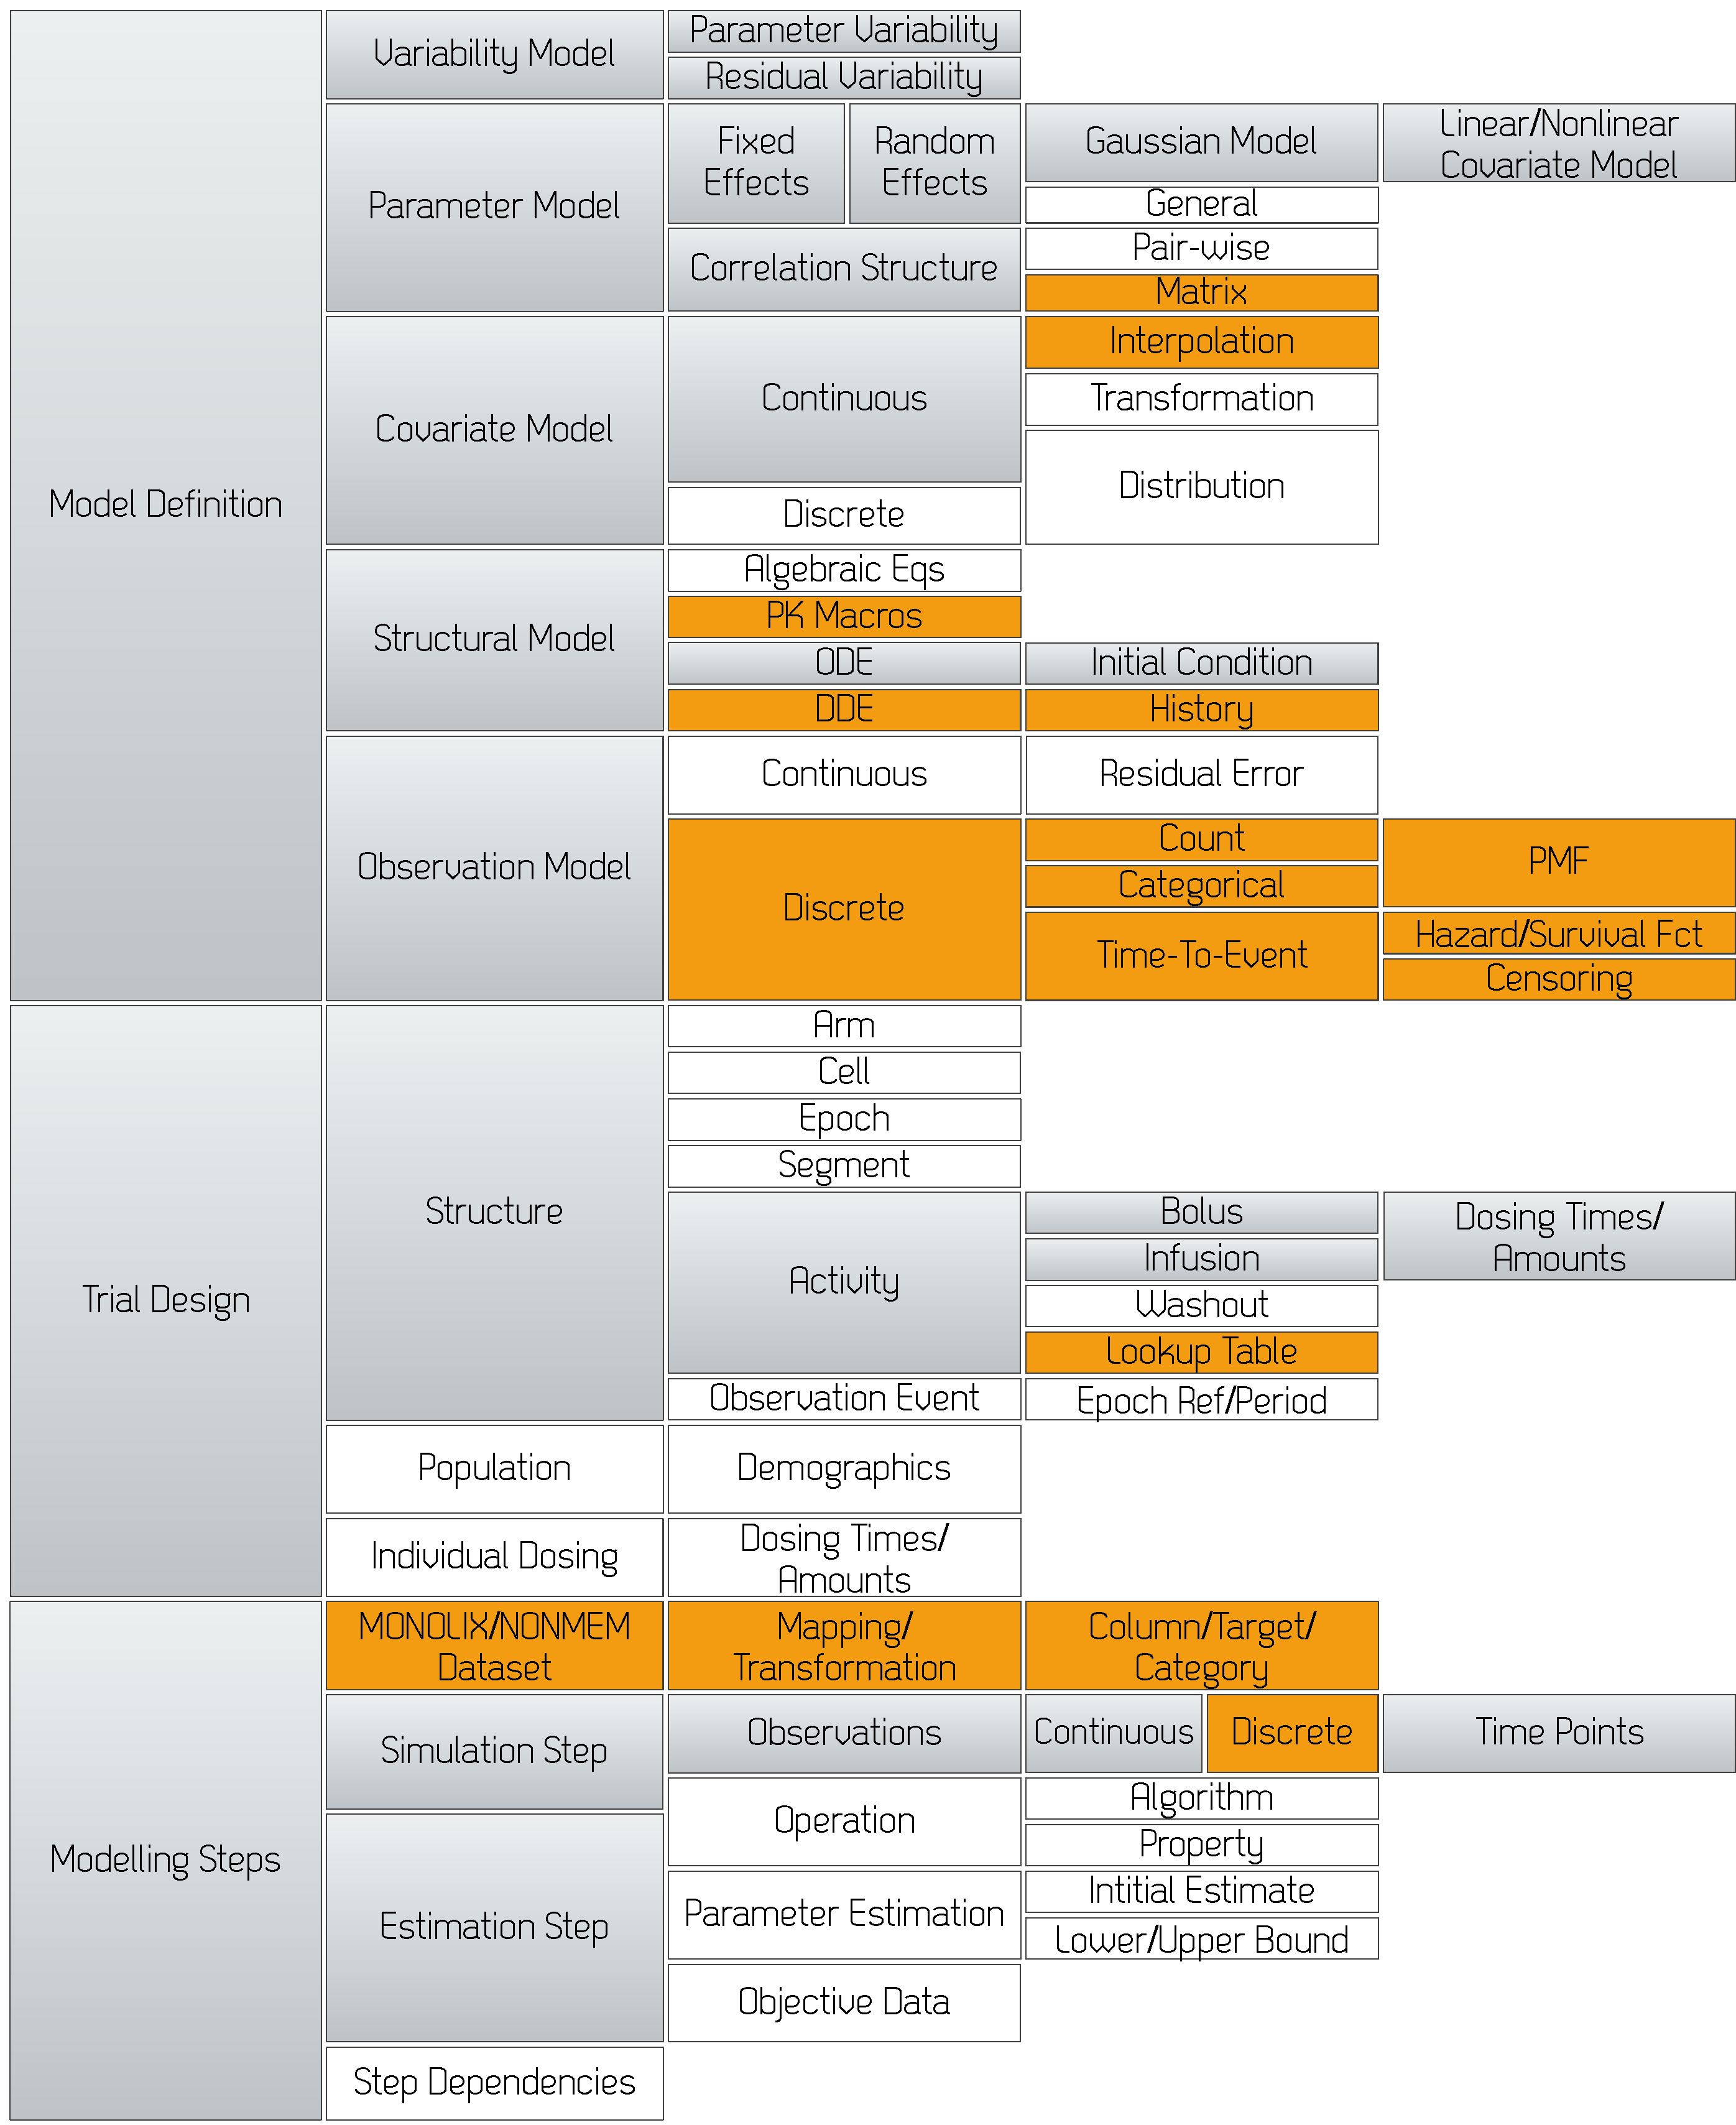
\includegraphics[height=0.85\textheight]{pics/PharmMLschemaOverview} % OverviewOfPharmML
  \caption{An overview of the organisation of \pharmml. The green highlighted cells illustrate the 
  	new elements introduced in this specification compared to the first public version 0.2.1. 
	Orange elements indicate minor changes or extensions.}
  \label{fig:momloverview}
\end{figure}

\subsection{Model Definition}

The \emph{Model Definition} defines the model, typically a population
model, that describes the system under investigation and any variability
between individuals in the population. The modeller may wish to use
it for simulation, parameter estimation or other types of analysis and
exploration. The \emph{Model Definition} in turn is composed of another
set of ``models'' that describe specific aspects of the overall model
definition. These are described below.

\subsubsection{Variability Model}
\label{sec:variability_model}

Variability is the concept that underpins a pharmacometric model and
the \emph{Variability Model} enables us to describe this. Note that it
is possible to describe variability in a \pharmml model without
defining random variability, but by using covariates.
Therefore the use of the \emph{Variability Model}
is optional. In \pharmml you can use this to define
individual random variability, but also a hierarchy of variability
above and/or below the level of the individual (e.g.\xspace inter-occasion
variability). For more details of the theory behind the random
variability model, see section \ref{sec:variabilityModel}.


\subsubsection{Covariate Model}

The \emph{Covariate Model} describes the covariates, both continuous and discrete, 
to be used in the \emph{Parameter Model} (figure \ref{fig:momloverview}). 
This defines a transformation, interpolation or probability distribution 
for a covariate. The formal description of the covariate
model can be found in section \ref{maths:covariate_model}.

\subsubsection{Parameter Model}

The \emph{Parameter Model} principally describes the parameters of the model
definition and is typically used to describe parameters with some
level of variability (typically between subject variability). The
parameter is defined more formally in section
\ref{maths:parameter_defn}, but essentially for each parameter we
define a population term, one or more random effects, and its
relationship to the covariates defined in the covariate model. The
random effects can be defined at different levels of variability
(defined by the variability model, see section
\ref{sec:variability_model}), which includes capturing their correlation
structure by providing a covariance (or correlation)
matrix for each level of variability.

\subsubsection{Structural Model}

At the heart of the model definition are one or more \emph{Structural
Model}s. These describe the system or systems that a modeller is
interested in and they represent a particular abstraction of that
system. For example a structural model may be used to describe the
pharmacokinetics of a drug. We can represent PK, PD or PK-PD models as
combinations of ODEs and algebraic equations. For compartmental
PK models an alternative coding options are the PK macros, as described
in the chapter \ref{sec:PKMacros}.
\subsubsection{Observation Model}

In clinical trials experimental observations are made, and these
observations are subject to experimental error. Different types of
instrument, assay or material sampled will all have different
statistical errors associated with them. In a pharmacometric model
these errors are described using a residual error model (see
section~\ref{maths:error_model}). In \pharmml we encode the residual
error model using the \emph{Observation Model}.


The outcomes of a clinical trial that we wish to model are not always
experimental measurements. A trial may aim to determine the efficacy
of an analgesic using a pain score provided by the subject; or measure
the frequency of seizure based on the maximum drug concentration; or
establish the remission rate over a given time in a cancer trial
\cite{Bonate:2011fk}. In each of these cases one needs to use a
discrete statistical model to represent these outcomes. These are also
defined in the Observation Model.

\subsection{Trial Design}
\label{sec:trialdesign_model}

Clinical trials are carefully structured and can vary considerably in
their complexity. Typically, a trial will be structured into one or
more arms with each arm subject to one or more treatment regimens
and observation protocols. Each arm is then populated with individuals
from a population of subjects who have been screened for their
suitability to participate in the trial. In \pharmml we have two options: 1)
the NONMEM/Monolix dataset to inform the model about the 
design, dosing and observation records, 2) \xelem{TrialDesign} section is used 
to describe the trial structure and subject population explicitly.
The latter option is a novel approach making the clinical trial much clearer 
to document, easier to encode computationally and to use for simulations 
or optimal design. More information can be found in chapter~\ref{sec:CTS}.

\begin{figure}[htb!]
 \centering
  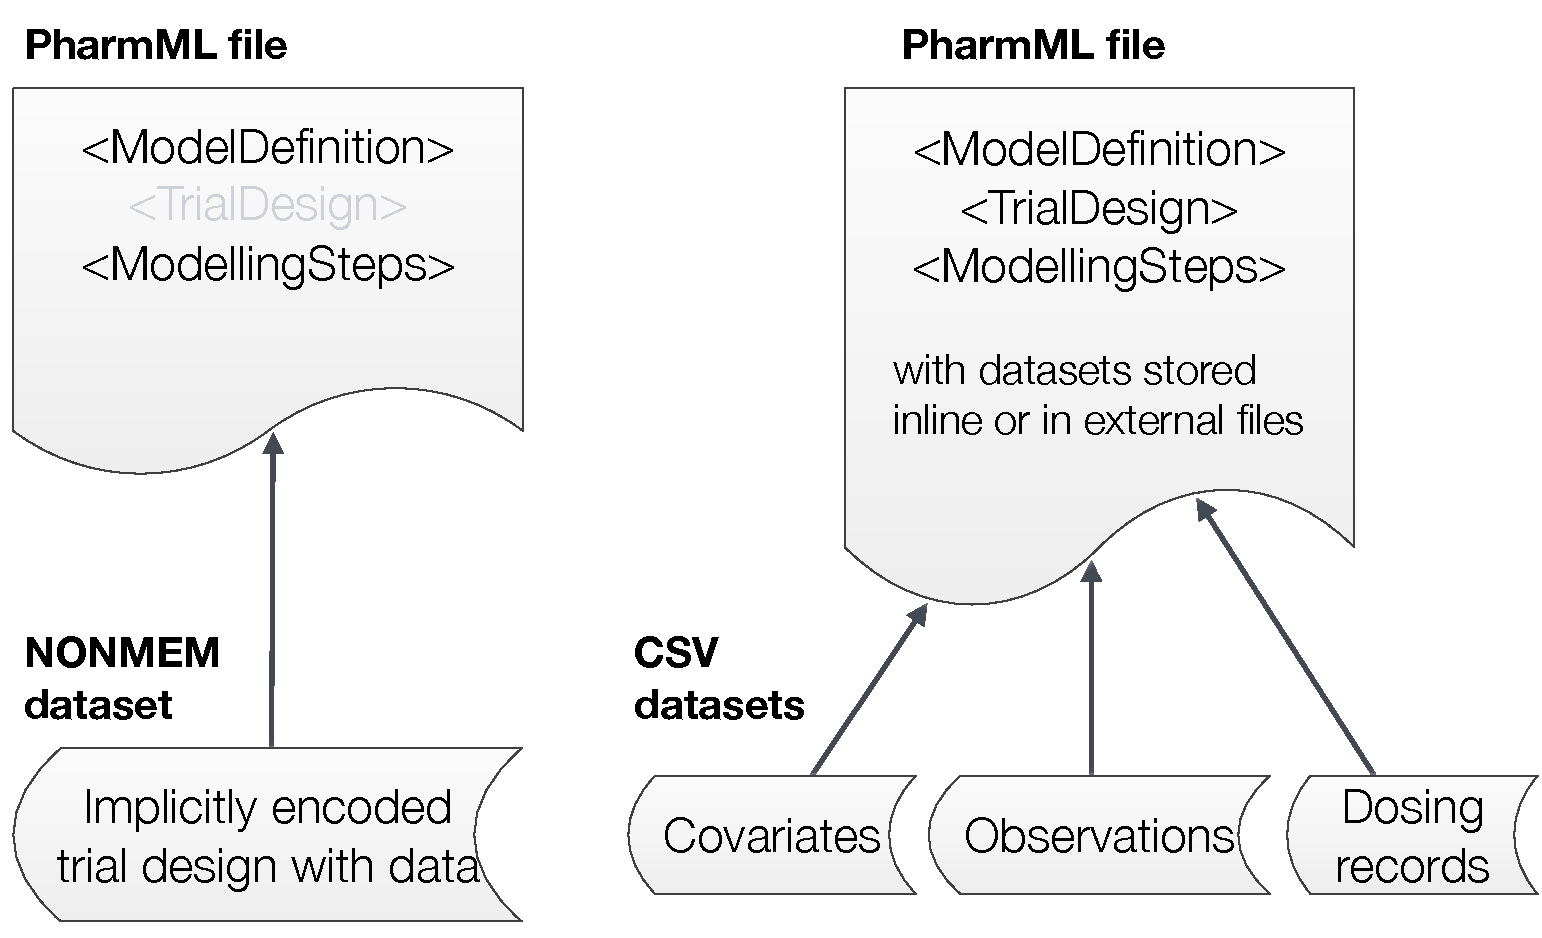
\includegraphics[width=0.5\textheight]{pics/DataVersusTrialDesign}
  \caption{Alternative ways to work with \pharmml -- either the information about the 
  underlying trial design and experimental records are sourced from a NONMEM type
  dataset or the trial design structure is encoded explicitly with datasets (covariates, 
  observation and dosing records) stored inline within the \pml model file or external 
  CSV files, see also Figure \ref{fig:dataStudyTaskFlow} for more details.}
  \label{fig:DataVersusTrialDesign}
\end{figure}

\begin{figure}[htb!]
 \centering
  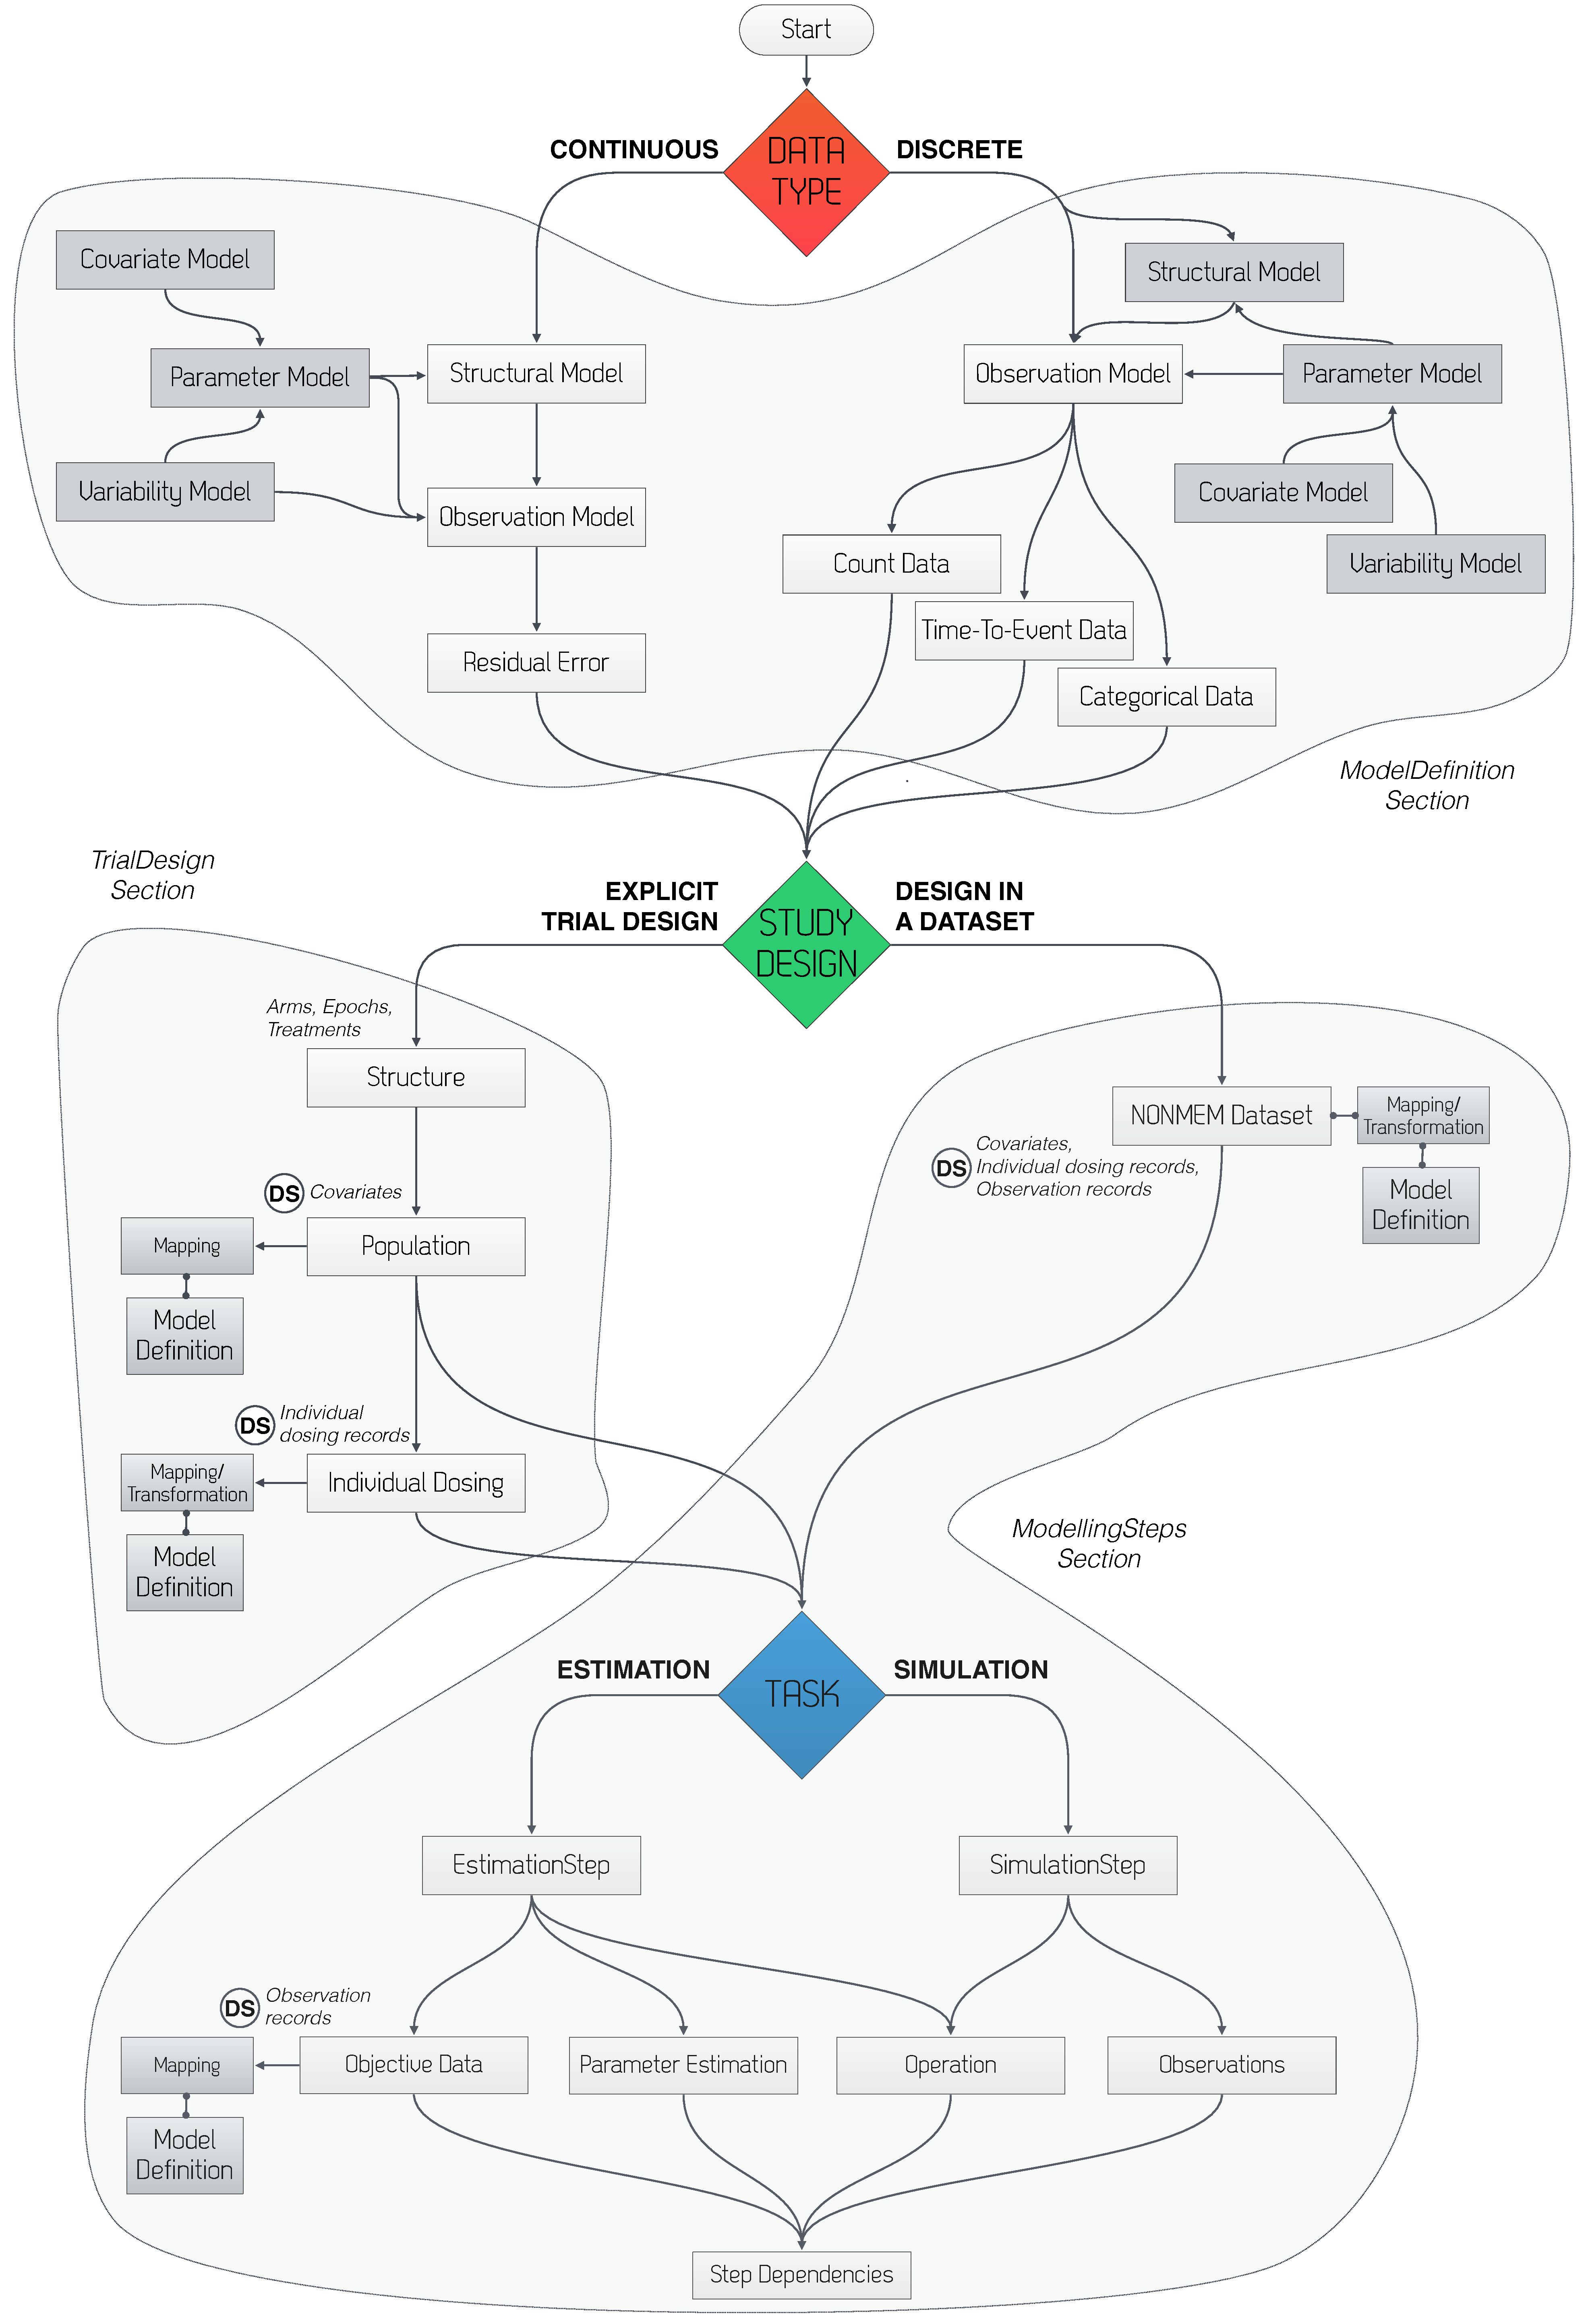
\includegraphics[height=0.90\textheight]{pics/Flowchart-dataTypeStudyTask}
  \caption{Working with \pharmml -- schema showing three essential decision points:
  the type of data (continuous and discrete), the source of the study design and data 
  (NONMEM dataset or \xelem{TrialDesign}) and finally the task type 
  (for now only simulation and estimation tasks are supported).}
  \label{fig:dataStudyTaskFlow}
\end{figure}

%%%%%%%%%%%%%%%%%%%%%%%%%%%%%%%%%%%%%%%%%%%%%%%%%%%%%%%%%%%%%%%%%%%%%%
\subsection{Modelling Steps}
\label{sec:stepdeps}
The final element when describing an M\&S experiment, after defining
the model and the associated trial design, is to describe how the
model was used. This section of a \pharmml document is akin to the
Methods section of a paper. The aim is not to replicate your modelling
exactly, but to provide enough information to reproduce the
model\footnote{To replicate the execution of a model requires detailed
  information about not only what algorithms were used to simulate or
  execute a model, but also what software implementation was used and
  exact supporting libraries such as that of the random number
  generator.}.

%%%%%%%%%%%%%%%%%%%%%%%%%%%%%%%%%%%%%%%%%%%%%%%%%%%%%%%%%%%%%%%%%%%%%%
\section{Identifiers, references and namespaces}

In \pharmml we use the Object Identifier \xatt{oid} to identify components in the
\emph{Trial Design} and \emph{Modelling Steps} sections of a \pharmml document and
the Symbol Identifier \xatt{symbId} to identify parameters and variables within the
\emph{Model Definition} section. Below we will describe the rules associated
with how they are defined and referenced.


%%%%%%%%%%%%%%%%%%%%%%%%%%%%%%%%%%%%%%%%%%%%%%%%%%%%%%%%%%%%%%%%%%%%%%
\subsection{Object identifiers}

The concept of the Object Identifier is borrowed from the CDISC XML
description of a trial design \cite{CDISC:2011a}. There they use the
attribute \xatt{oid} to identify and to reference components used in
the design. Object identifiers have global scope, which means that all
object identifiers defined in a \pharmml document must be unique.

Elements that reference an object identifier by convention use the
attribute \texttt{oidRef} and the id referred to must exist in the
\pharmml document. In addition the object referred to must be
compatible with the element referencing it. The example below shows
how this works:
%
\lstset{language=XML}
\begin{lstlisting}
<Epoch oid="e1">
  <!-- Detail omitted -->
</Epoch>
<Arm oid="a2">
  <!-- Detail omitted -->
</Arm>
<Cell oid="c2">
    <EpochRef oidRef="e1" />
    <ArmRef oidRef="a2"/>
    <SegmentRef oidRef="tb"/>
</Cell>
\end{lstlisting}
%
Here the element \xelem{EpochRef} refers to the object identifier of
the Epoch, ``e1'', and the \xelem{ArmRef} element refers to the Arm
object, ``a2''. This is correct. However, the following example
is incorrect:
%
\lstset{language=XML}
\begin{lstlisting}
<Epoch oid="e1">
  <!-- Detail omitted -->
</Epoch>
<Arm oid="a2">
  <!-- Detail omitted -->
</Arm>
<Cell oid="c2">
    <!-- ERROR: not valid PharmML -->
    <EpochRef oidRef="a2" />
    <ArmRef oidRef="a2"/>
    <SegmentRef oidRef="tb"/>
</Cell>
\end{lstlisting}
%
The \xelem{EpochRef} points to the Arm object, which is not compatible
with it. Note that this cannot be validated using SML Schema. 
These compatibilities are documented for each element
containing an object reference (i.e.\xspace an \xatt{oidRef}
attribute) in the XML Schema. 


%%%%%%%%%%%%%%%%%%%%%%%%%%%%%%%%%%%%%%%%%%%%%%%%%%%%%%%%%%%%%%%%%%%%%%
\subsection{Blocks and symbol scoping}
\label{sec:blocks}
\label{sec:scoping-rules}

\pharmml defines names for the
parameters, variables and parts of the model that need to be uniquely
identified. In \pharmml we refer to these collectively as symbols. The
rules we apply are relatively simple in that all symbols within a
\pharmml document must be unique and that all symbols in the document are
`visible'. In other words a symbol defined in one part of a document
will be available to a component elsewhere in the document. Symbols in
\pharmml can be organised into different scopes, which in turn are
defined by blocks. We illustrate this conceptually in the example
below\footnote{Note that in the example we use the element
  \xelem{Symbol} to define a symbol and \xelem{Block} a block. These
  are not actually valid \pharmml elements, but we hope to make the
  scoping discussion clearer by using these.}:

\lstset{language=XML}
\begin{lstlisting}
<Block blkId="blockID">
	...
	<Symbol symbId="symbolID">
		...
	</Symbol>
	...
        <SymbRef symbIdRef="symbolID"/>
</Block>

<ElsewhereInXMLDocument>
	<SymbRef blkIdRef="blockID" symbIdRef="symbolID"/>
</ElsewhereInXMLDocument>
\end{lstlisting}
The block is given an identifier and is used to organise symbols. Any
symbols that are defined within it are part of the block's scope (private symbols). If
we refer to that symbol within the block then we do not need to specify the
block name. When referred to outside the block, then the same symbol
must be referred to using a combination of the block identifier
(\xatt{blkId}) and symbol identifier (\xatt{symbId}). This is illustrated
more completely in the example below:

\lstset{language=XML}
\begin{lstlisting}
<Symbol symbId="symb2"/> <!-- Decl 1 -->
<Symbol symbId="symb3"/> <!-- Decl 2 -->

<Block blkId="A">
	<Symbol symbId="symb2"/> <!-- Decl 3 -->
        <SymbRef symbIdRef="symb2"/> <!-- resolves to Decl 3 -->
        <SymbRef symbIdRef="symb3"/>  <!-- resolves to Decl 2 -->
</Block>

<Block blkId="B">
	<Symbol symbId="symb2"/>  <!-- Decl 4 -->
	<Symbol symbId="symb3"/> <!-- Decl 5 -->
        <SymbRef symbIdRef="symb2"/>  <!-- resolves to Decl 4 -->
</Block>

<ElsewhereInXMLDocument>
	<SymbRef symbIdRef="symb2"/> <!-- resolves to Decl 1 -->
	<SymbRef blkIdRef="A" symbIdRef="symb2"/> <!-- resolves to Decl 3 -->
	<SymbRef blkIdRef="B" symbIdRef="symb2"/> <!-- resolves to Decl 4 -->
	<SymbRef blkIdRef="B" symbIdRef="symb3"/> <!-- resolves to Decl 5 -->
</ElsewhereInXMLDocument>
\end{lstlisting}

Here, the \xelem{Symbol} element defines a symbol and \xelem{SymbRef}
refers to it.  As you can see, a symbol can be defined in several
places: globally (outside a block) and within blocks A and B. In each
case identical \xatt{symbID}s are used, but the language can
distinguish between them because of the context. This is clear when we
look at the symbol references in the \xelem{ElsewhereInXMLDocument}
element. Referring to a symbol, for example symbol \attval{symb2} in
block A may seem ambiguous, but the scoping rules of \pharmml are
clear. The reference is resolved first to the scope within the block
and then to the global scope. So in block A the reference to
\attval{symb2} points to Decl 3, and the reference to \attval{symb3}
points to the global symbol, Decl 2 and not Decl 5, which is a
different scope. These scoping rules are common to many programming
languages. One question you may ask is what if a globally defined symbol
has the same name as a block identifier? This is handled by the
symbol namespace rules. Both types of identifier share the same (global)
namespace and so cannot have the same name.

You will notice in the discussion above that we use the words `define'
and `reference'. These are important concepts in \pharmml. Symbols can be
\emph{defined} only once, but can be \emph{referred} to many
times. Symbols can be referred to before they are defined. 
\pharmml is a declarative language (unlike C or Fortran), thus it is natural
that the order of variable definition is not important. The listing below
shows how this works using real \pharmml.

\lstset{language=XML}
\begin{lstlisting}
<ct:Variable symbId="c" symbolType="real">
    <ct:Assign>
        <Equation xmlns="http://www.pharmml.org/pharmml/0.6/Maths">
            <Binop op="divide">
                <ct:SymbRef symbIdRef="b"/>
                <ct:Real>10</ct:Real>
            </Binop>
        </Equation>
    </ct:Assign>
</ct:Variable>
<ct:Variable symbId="a" symbolType="real">
    <ct:Assign>
        <Equation xmlns="http://www.pharmml.org/pharmml/0.6/Maths">
            <Binop op="plus">
                <ct:SymbRef symbIdRef="b"/>
                <ct:SymbRef symbIdRef="c"/>
            </Binop>
        </Equation>
    </ct:Assign>
</ct:Variable>
<ct:Variable symbId="b" symbolType="real">
    <ct:Assign>
        <ct:Real>1</ct:Real>
    </ct:Assign>
</ct:Variable>
\end{lstlisting}

One danger with this approach is that the language syntax does not
prevent the creation of cyclic dependencies between variables. An
example of this is shown below where there is dead-lock because neither variable can be initialised
because the other is yet to be defined. Such cycles are forbidden in
\pharmml and must be checked for when validating the language.
(See section \ref{subsec:AssinmentRules} with the description of related
validation rules, which are already or are supposed to be implemented 
and handled by 
libPharmML\footnote{\url{https://sourceforge.net/projects/libpharmml.ddmore.p}}, 
an API under development as part of the DDMoRe project.)
\lstset{language=XML}
\begin{lstlisting}
<!-- ERROR: The declaration below creates a cycle -->
<ct:Variable symbId="d" symbolType="real">
    <ct:Assign>
        <ct:SymbRef symbIdRef="e"/>
    </ct:Assign>
</ct:Variable>
<ct:Variable symbId="e" symbolType="real">
    <ct:Assign>
        <ct:SymbRef symbIdRef="d"/>
    </ct:Assign>
</ct:Variable>
\end{lstlisting}

Related to variable definition is the initialisation of a symbol: also
known as initial assignment. When a symbol is defined it is in an
uninitialised state and has no value. It may be either initialised
during the definition, as in the examples above, or via a subsequent
initial assignment as below:

\lstset{language=XML}
\begin{lstlisting}
<!-- Symbol defined, but not initialised -->
<ct:Variable symbId="a" symbolType="real"/>
<!--  Omitted detail -->
<ct:VariableAssignment>
    <ct:SymbRef  symbIdRef="a"/>
    <ct:Assign>
        <math:Equation>
            <math:Binop op="plus">
                <ct:SymbRef symbIdRef="a"/>
                <ct:Real>10</ct:Real>
            </math:Binop>
        </math:Equation>
    </ct:Assign>
</ct:VariableAssignment>
\end{lstlisting}

Either way this can only be done once. This listing illustrates the problem:
\lstset{language=XML}
\begin{lstlisting}
<!-- Symbol defined, but not initialised -->
<ct:Variable symbId="a" symbolType="real"/>
<!-- Snip -->

<!-- Incorrect -->
<!-- Duplicate initial assignments here. -->
<ct:VariableAssignment>
    <ct:SymbRef  symbIdRef="a"/>
    <ct:Assign>
        <ct:Real>0</ct:Real>
    </ct:Assign>
</ct:VariableAssignment>
<ct:VariableAssignment>
    <ct:SymbRef  symbIdRef="a"/>
    <ct:Assign>
        <math:Equation>
            <math:Binop op="plus">
                <ct:SymbRef symbIdRef="a"/>
                <ct:Real>10</ct:Real>
            </math:Binop>
        </math:Equation>
    </ct:Assign>
</ct:VariableAssignment>
\end{lstlisting}
\pharmml is a declarative language and the order is not important, 
thus symbols in \pharmml can only be initialised
once.


Note that in \pharmml symbol references between sections only go in one
direction. All sections point to the \emph{Model Definition}, but not
the reverse and the \emph{Modelling Steps} section points to the
\emph{Trial Design} section, but again not \emph{vice
  versa}\xspace. By maintaining this layered dependency structure in
the design of \pharmml we simplify the design of the language and ensure
that the \emph{Model Definition} section is guaranteed to be
independent of the other \pharmml sections.

\subsection{Interaction between Object and Symbol identifiers}

The Object and Block identifier (\xatt{oid} and \xatt{blkId}
respectively) both exist in the same \pharmml document and they share
the same namespace. This means that they cannot share the same
identifier, as is illustrated below:
%
\lstset{language=XML}
\begin{lstlisting}
<Symbol symbId="symb2"/>

<Block blkId="A"> <!-- ERROR -->
	<Symbol symbId="symb3"/>
</Block>

<Block blkId="B"> <!-- OK -->
	<Symbol symbId="symb4"/>
</Block>

<Oid oid="A"/> <!-- ERROR -->
<Oid oid="Z"/> <!-- OK -->
<Oid oid="symb2"/> <!-- ERROR -->
<Oid oid="symb3"/> <!-- OK -->
\end{lstlisting}
%
Similarly, just as a global \xatt{symbId} cannot share an identifier with a
\xatt{blkId} (see section~\ref{sec:scoping-rules}), neither can it
share an identifier (in the above case ``symb2'') with an \xatt{oid}.


%%%%%%%%%%%%%%%%%%%%%%%%%%%%%%%%%%%%%%%%%%%%%%%%%%%%%%%%%%%%%%%%%%%%%%
\section{Type checking}
\label{sec:type-checking}

Symbols in \pharmml have a type. By symbol we mean something defined
using a \xatt{symbId} attribute (for example a variable or
parameter). Like a variable a type is simply a way we use in \pharmml to
map symbols to an abstraction: such as a number, a string or a table
of values. As you might expect, symbols with different types are not
always compatible with each other, so it is necessary when validating
the correctness of a \pharmml document to ensure that the types of its
symbols are compatible with each other. This is known as type checking
(see \cite[Chapter6]{Aho:1986fk} and \cite[Chapter 8]{Parr:2010uq} for
more information). The types in \pharmml are enumerated in table
\ref{tab:type-specification}.


The types used in \pharmml must be consistent. In general this means that
all types in an expression should be identical. This is illustrated in
the following example:
%
\lstset{language=XML}
\begin{lstlisting}
<!-- ERROR: incompatible type -->
<ct:Variable symbId="a" symbolType="int">
    <ct:Assign>
        <ct:String>A value</ct:String>
    </ct:Assign>
</ct:Variable>
<ct:Variable symbId="b" symbolType="boolean"/>
<ct:Variable symbId="c" symbolType="real">
    <ct:Assign>
        <m:Equation>
            <m:Binop op="plus"> <!-- ERROR: Cannot add a real to a Boolean -->
                <ct:Real>22</ct:Real>
                <ct:SymbRef symbIdRef="b"/>
            </m:Binop>
        </m:Equation>
    </ct:Assign>
</ct:Variable>
<ct:Variable symbId="d" symbolType="real">
    <ct:Assign>
        <ct:Int>453</ct:Int> <!-- OK -->
    </ct:Assign>
</ct:Variable>
\end{lstlisting}
%
Note that the variable $d$ is of type real but was
initialised with an integer value, and that this was permitted. This
is an exception to the rule that all types must be the same and is
a common mechanism in computer languages, called type promotion. Here
the integer value can be converted to a real with no loss of
information and so it is permitted. The reverse conversion is not
permitted because a real value may lose information when converted to
an integer.


%%%%%%%%%%%%%%%%%%%%%%%%%%%%%%%%%%%%%%%%%%%%%%%%%%%%%%%%%%%%%%%%%%%%%
\section{Two ways to connect trial design and model}
\label{subsec:twoModes}
There are two basic options\footnote{In version 0.2.1 only the \xelem{TrailDesign}
based option was supported. This however proved to be very limiting for 
various reasons and support for NONMEM/Monolix datasets has been required.}  
to provide trial design related information in \pml. In the first the entire information 
is implemented in the \pml file, while in the second datasets with experimental 
data are used, see Figure \ref{fig:DataVersusTrialDesign} and \ref{fig:dataStudyTaskFlow}.

\begin{table}[h!]
\setlength{\tabcolsep}{15pt}
\begin{center}
\begin{tabular}{ll}
  \hline
 \xelem{TrialDesign} and inline datasets & External NONMEM dataset \\
  \hline
  \lstset{language=XML}
\begin{lstlisting}
<ModelDefinition>
    ...
</ModelDefinition>
<TrialDesing>
    <Structure>
        ...
    </Structure>
    <Population>
        ...
    </Population>
</TrialDesing>
<ModellingsSteps>
    <EstimationStep oid="est1">
        <ObjectiveDataSet>
            ...
        </ObjectiveDataSet>                
        ...
    </EstimationStep>
    ...
</ModellingsSteps>
\end{lstlisting}
&
\lstset{language=XML}
\begin{lstlisting}
<ModelDefinition>
    ...
</ModelDefinition>

<!-- TrailDesign section is not required -->

<ModellingsSteps>
    <ExternalDataSet toolName="NONMEM" oid="DSoid">
        ...
    </ExternalDataSet>
    
    <EstimationStep oid="est1">
        <ExternalDataSetReference>
            <ct:OidRef oidRef="DSoid"/>
        </ExternalDataSetReference>
        ...
    </EstimationStep>
    ...
</ModellingsSteps>
\end{lstlisting}  
\\
    \hline
\end{tabular}
\caption{Comparison of model structures encoded using \xelem{TrialDesign} 
(left) and using NONMEM format dataset (right). In the latter case the 
\xelem{TrialDesign} part is redundant and the complete information about 
the study design is sourced from the dataset. This holds for both estimation and 
simulation tasks.}
\label{tab:withAndWithoutNM}
\end{center}
\end{table}

Table \ref{tab:withAndWithoutNM} shows the \pml code for these two options 
as described in the following
\begin{itemize} 
\item
Using \xelem{TrialDesign}/\xelem{ModellingSteps} -- trial design (information about 
design arms, dosing times, amounts etc.) is encoded explicitly in XML and according 
experimental data records are provided within three datasets.
More specifically covariates and individual dosing records are encoded in 
the \xelem{Population} element of the \xelem{TrialDesign} section, while the
observation records, in \pml referred to as \xelem{ObjectiveDataSet}, are stored 
in \xelem{ModellingSteps}, see Table \ref{tab:withAndWithoutNM} (left).
\item
Using NONMEM/Monolix datasets -- these files contain the complete information 
about the underlying trial design, both for estimation or simulation tasks. 
Using datasets has consequences for the content of the \pml document 
in that the \xelem{TrialDesign} part is in such case redundant. Instead the dataset
is referenced in the \xelem{ExternalDataSet} element and referenced later in e.g.
estimation task, \xelem{ExternalDataSetReference}, see Table \ref{tab:withAndWithoutNM}
(right).
\end{itemize}


%%%%%%%%%%%%%%%%%%%%%%%%%%%%%%%%%%%%%%%%%%%%%%%%%%%%%%%%%%%%%%%%%%%%%%
\section{Datasets}
\label{sec:datasets}

The dataset is a key concept in PharmML and is used to describe the data 
of the relevant trial design, i.e. the observations, covariates and dosing
records. 
The data is tabular and the dataset has therefore been designed to 
represent this type of information and all data is explicitly typed.


%%%%%%%%%%%%%%%%%%%%%%%%%%%%%%%%%%%%%%%%%%%%%%%%%%%%%%%%%%%%%%%%%%%%%%
\subsection{Inline datasets}
\label{subsec:inlineDataset}
We start with the data implemented entirely within the \pml file. As usual 
the simplest way to explain it is to look at an example, such as the code 
snippet below:
\lstset{language=XML}
\begin{lstlisting}
<ds:DataSet>
    <ds:Definition>
        <ds:Column columnId="id" columnType="id" valueType="string" columnNum="1"/>
        <ds:Column columnId="arm" columnType="arm" valueType="string" columnNum="2"/>
        <ds:Column columnId="reps" columnType="replicate" valueType="int" columnNum="3"/>
    </ds:Definition>
    <ds:Table>
        <ds:Row>
            <ct:String>i1</ct:String><ct:String>a1</ct:String><ct:Int>20</ct:Int>
        </ds:Row>
        <ds:Row>
            <ct:String>i2</ct:String><ct:String>a2</ct:String><ct:Int>20</ct:Int>
        </ds:Row>
        <ds:Row>
            <ct:String>i3</ct:String><ct:String>a3</ct:String><ct:Int>40</ct:Int>
        </ds:Row>
        <ds:Row>
            <ct:String>i4</ct:String><ct:String>a4</ct:String><ct:Int>40</ct:Int>
        </ds:Row>
    </ds:Table>
</ds:DataSet>
\end{lstlisting}
%
The dataset starts with \xelem{Definition} where the columns of the
dataset table are defined. For each column the following attributes have to be 
specified
\begin{itemize} 
\item
\xatt{columnId} -- the name of the column  
\item
\xatt{columnType} --  the type of the column identifies 
the role the stored item plays in the model, see Table \ref{tab:MDLPharmML_columnTypes}
for the explanation of allowed values.  

\item
\xatt{valueType} -- the type of each column value is specified, which
complies with the \pharmml type system.  
\item
\xatt{columnNum} -- the column number must start at 1 and each
column must be numbered in consecutive order (i.e.\xspace 1,2,3,4\ldots etc.). 
\end{itemize}
Next the content of the dataset is held within the \xelem{Table} element and 
this consists of one or more \xelem{Row} elements. Each row must contain 
an entry for each column defined. This approach is based on the concept of 
a relation in relational theory. Therefore the ordering of rows is not significant. 

\begin{table}[ht!]
\begin{center}
\begin{tabular}{ll}
  \hline
\xatt{columnType} & Meaning \\  
  \hline
addl  & number of additional doses     \\
adm  & type of administration     \\
arm &     study arm \\
censoring  & left-censored data     \\
covariate  & covariates     \\
cmt & target compartment \\
demographic &     demographic type \\
dose  & dose      \\
duration & infusion duration \\
dv  & dependent variable     \\
dvid  & mixed observations     \\
epoch &     study epoch \\
evid  &  dose events     \\
id   & subject identifiers      \\
idv   & independent variable     \\
ii   & inter-dose interval     \\
limit  & lower limit for interval-censored data     \\
mdv  & missing dependent variable     \\
occasion   & occasions     \\
rate   & infusion rate     \\
reg   & regression variable     \\
replicate &     in cases when subjects are assumed identical \\
ss   & steady state \\
ssEndTime &     steady-state administration end time \\
ssPeriod &     steady-state administration interval \\
time  & time     \\
undefined & value for any undefined cases \\
   \hline
\end{tabular}
\caption{A summary of allowed values for the \xatt{columnType} attribute in \pml.}
\label{tab:MDLPharmML_columnTypes}
\end{center}
\end{table}


%%%%%%%%%%%%%%%%%%%%%%%%%%%%%%%%%%%%%%%%%%%%%%%%%%%%%%%%%%%%%%%%%%%%%%
\subsection{NONMEM/Monolix datasets}
\label{subsec:externalDataset}
Inline storage of data split into three tables has disadvantages in that 
it requires provision of additional translation tools to convert standard 
datasets to this format. Editing such data sets by hand is 
very error prone and time consuming.

There was a lot of request for supporting external datasets, more specifically
those used by NONMEM, Monolix and other tools. 
As shown in the following listing, the external data set can be specified using the 
new \xelem{ImportData} element, instead of \xelem{Table}, by providing the file 
path relative to the \pml file. Optional parameters such as file format and 
delimiter can also be provided. The external file must be a valid input file for the target tool.
%\emph{CSV}, with four delimiters: \xatt{COMMA}, \xatt{SEMICOLON}, \xatt{SPACE} 
%and \xatt{TAB}. 
The template for this reads: 
\lstset{language=XML}
\begin{lstlisting}
    <ds:ExternalFile oid="id1">
        <ds:path>FILE_PATH</ds:path>
        <ds:format>FORMAT</ds:format>
        <ds:delimiter>DELIMITER_TYPE</ds:delimiter>
    </ds:ExternalFile>
    \end{lstlisting}
And listing below shows a simple example how this works. As before the \xelem{Definition}
defines the table content and a reference to the according file and its type is provided.
\lstset{language=XML}
\begin{lstlisting}
    <ds:DataSet>
        <ds:Definition>
            <ds:Column columnId="ID" columnType="id" valueType="id" columnNum="1"/>
            <ds:Column columnId="ARM" columnType="arm" valueType="id" columnNum="2"/>
            <ds:Column columnId="SEX" columnType="covariate" valueType="id" columnNum="3"/>
            <ds:Column columnId="EPOCH" columnType="epoch" valueType="id" columnNum="4"/>
        </ds:Definition>
    	<ds:ExternalFile oid="id1">
	    <ds:path>warfarin_conc_pca.csv</ds:path>
            <ds:format>CSV</ds:format>
            <ds:delimiter>COMMA</ds:delimiter>
        </ds:ExternalFile>
    </ds:DataSet>
\end{lstlisting}

%%%%%%%%%%%%%%%%%%%%%%%%%%%%%%%%%%%%%%%%%%%%%%%%%%%%%%%%%%%%%%%%%%%%%%
\subsection{\xelem{TrialDesign} external datasets}
\label{subsec:TrialDesignExternal}

In the \xelem{TrialDesign} section the user has the choice between inline or
external dataset storage, see Section \ref{sec:trialdesign_model}.
External datasets can be specified using the \xelem{ImportData} element. 
As shown in the example below, you must provide the file path relative to the PharmML file, 
file format (only CSV files allowed) and one of the allowed delimiters (\xatt{COMMA}, 
\xatt{SEMICOLON}, \xatt{SPACE}, \xatt{TAB}). Further validation rules are listed in xxx.

\lstset{language=XML}
\begin{lstlisting}
            <ds:ExternalFile oid="id1">
                <ds:path>/datasets/myData.csv</ds:path>
                <ds:format>CSV</ds:format>
                <ds:delimiter>COMMA</ds:delimiter>
            </ds:ExternalFile>
\end{lstlisting}



%%%%%%%%%%%%%%%%%%%%%%%%%%%%%%%%%%%%%%%%%%%%%%%%%%%%%%%%%%%%%%%%%%%%%%
\subsection{Lookup table}
\label{subsec:lookupTable}

\xelem{TrialDesign} can be used to define a wide range of dosing scenarios 
which can be used to encode virtually any PK model. Sometimes however, 
the concentration data we want to couple with a PD model is available as a 
lookup table, i.e. PK measurement records for which the underlying model 
is unknown or not required.

First the data has to be implemented and this is done using the \xelem{LookupTable}
element within the \xelem{Activity} of the \xelem{TrialDesign}. The target variable 
in the model needs to be defined and finally an interpolation algorithm chosen 
from a build-in list with the most common choices, i.e. constant, linear, nearest, 
spline, pchip and cubic. There are of course other scenarios when a lookup table is 
useful, e.g. in the minimal model where the measured insulin is provided in tabular
format.


%%%%%%%%%%%%%%%%%%%%%%%%%%%%%%%%%%%%%%%%%%%%%%%%%%%%%%%%%%%%%%%%%%%%%%
\subsection{Dataset mapping and scaling}
\label{subsec:lookupTable}

The provision of a dataset, implemented as inline data, as external files or 
as lookup tables is not sufficient to make it work. What is additionally required 
is a set of consistent rules and structure for the mapping between 
various model elements (such as administration targets, continuous/discrete 
observations, continuous/discrete covariates, categories in discrete models, 
occasions) and data records. The same holds for mapping between above 
mentioned model elements and various administration options as defined 
in \xelem{TrialDesign}. We will see lots of examples for such mappings in 
Chapter \ref{chap:worked-egs}.

Similar holds for the dose adjustment, a very frequent element of a PK study, 
which is tightly coupled with column mapping. Typically such adjustment 
means scaling with respect to bodyweight, BW, or body surface area, BSA, 
or other continues covariates, such as creatine clearance, CLcr. We will discuss 
examples for such mappings which are defined in connection with the datasets 
in Chapter \ref{chap:worked-egs}.


%%%%%%%%%%%%%%%%%%%%%%%%%%%%%%%%%%%%%%%%%%%%%%%%%%%%%%%%%%%%%%%%%%%%%%
\section{Defining differential equations}
\label{sec:odes}

The easiest way to understand how one defines a differential equation in \pharmml
is to look at an example.

\begin{align*}
	\dfrac{\mathrm{d}\mathit{Ad}}{\mathrm{d}t}  &=  -\mathit{ka}\,  \mathit{Ad}, \quad \textit{Ad}(t=t_0)  =  A_0
\end{align*}
%
The corresponding \pharmml to the above equation is listed below:
%
\lstset{language=XML}
\begin{lstlisting}
            <ct:DerivativeVariable symbId="Ad" symbolType="real">
                <ct:Assign>
                    <Equation xmlns="http://www.pharmml.org/pharmml/0.6/Maths">
                        <Binop op="times">
                            <Uniop op="minus">
                                <ct:SymbRef blkIdRef="p1" symbIdRef="ka"/>
                            </Uniop>
                            <ct:SymbRef symbIdRef="Ad"/>
                        </Binop>
                    </Equation>
                </ct:Assign>
                <ct:IndependentVariable>
                    <ct:SymbRef symbIdRef="t"/>
                </ct:IndependentVariable>
                <ct:InitialCondition>
                    <ct:InitialValue>
                        <ct:Assign>
                            <ct:SymbRef symbIdRef="A0"/>
                        </ct:Assign>
                    </ct:InitialValue>
                    <ct:InitialTime>
                        <ct:Assign>
                            <ct:SymbRef symbIdRef="t0"/>
                        </ct:Assign>
                    </ct:InitialTime>
                </ct:InitialCondition>
            </ct:DerivativeVariable>
\end{lstlisting}


As you can see a derivative variable is defined using the
\xelem{DerivativeVariable} element and the right-hand side of the
equation is described by the \xelem{Assign} element. The independent
variable is explicitly defined in this example using the
\xelem{IndependentVariable}. If it had been omitted then the
derivative would have defaulted to the independent variable set for
the \pharmml document as a whole. Finally its initial condition is
set to a constant $A_0$ at $t_0$ in the \xelem{InitialCondition} element, but 
in fact any expressions are allowed in \xelem{InitialValue} and \xelem{InitialTime}. 
There are a few points to note about the definition of the derivative:
%
\begin{enumerate}
\item The symbol types on the RHS of the definition are a mixture of
  derivative variables and non-derivative variables and
  parameters. 
\item The definition of the variable $Ad$ contains a reference to
  itself. If this were the definition of a non-derivative type, then this
  would be regarded as a cyclic dependency and not be permitted, but
  in the definition of an ODE it is.
\end{enumerate}


%%%%%%%%%%%%%%%%%%%%%%%%%%%%%%%%%%%%%%%%%%%%%%%%%%%%%%%%%%%%%%%%%%%%%%
\subsection{Delayed differential equations}
\label{subsec:ddes}

The following new elements extend the ODE structure
\begin{itemize}
\item
\xelem{Delay} element with arguments
\begin{itemize}
\item
y, a model variable
\item
$\tau$, discrete delay, can be a numerical value or a symbol
\end{itemize}
\item
\xelem{History} element where the past of a variable is defined for $t \leq t_0$. 
It comes with two child elements
\begin{itemize}
\item
\xelem{HistoryValue} stands for past/historical value of a variable $y$, denoted by $y_0$.
\item
\xelem{HistoryTime} stands for the end time, t0, of the history definition. 
By default, history is defined for $t \leq t_0$.
\end{itemize}
\end{itemize}
Then the typical delay expression such as $y(t-\tau)$ would be encoded as
\lstset{language=XML}
\begin{lstlisting}
            <ct:Delay>
                <ct:SymbRef symbIdRef="y"/>
                <ct:DelayVariable >
                    <ct:SymbRef blkIdRef="pm1" symbIdRef="tau"/>
                </ct:DelayVariable>
            </ct:Delay>
\end{lstlisting}
with $\tau$ defined in the \xelem{ParameterModel} \emph{pm1}.


%%%%%%%%%%%%%%%%%%%%%%%%%%%%%%%%%%%%%%%%%%%%%%%%%%%%%%%%%%%%%%%%%%%%%%
\section{Mathematical expressions}
\label{sec:maths}
Mathematical expressions are a fundamental part of a pharmacometric
model and so it was important that \pharmml incorporated the
ability to encode these. The question we had in designing the language, however, was
what is the best way to do this?  Our initial approach was to reuse an
existing W3C standard called
\mathml\footnote{\url{http://www.w3.org/TR/MathML3/}}, which was
designed to represent mathematical equations on web pages.
Unfortunately, the full \mathml standard is bigger and more complex
than we need: indeed much of the standard focuses on the presentation
and layout of mathematical equations rather than their underlying
meaning\footnote{We should emphasise that his is not a criticism of
\mathml, as this was the problem it was created to solve!}.  This
was also the conclusion reached for similar standards to \pharmml such as
SBML \cite[Section 3.4]{sbmll3v1c},
CellML\footnote{\url{http://www.cellml.org/specifications/cellml_1.1/\#sec_mathematics}}
and \sedml \cite{sedmll1v1}. Their solution to this problem was to use
a subset of the standard that did what they wanted and to develop their
own software to support this subset. In effect they created their own
version of the \mathml standard. This means that the CellML version of
\mathml is not compatible with the \sbml version and so on, and as a
consequence each standard has had to develop its own software
libraries to support their own version of \mathml.

Faced with the same dilemma we considered adopting yet another subset
of \mathml, but decided against it for a number of reasons:
\begin{enumerate}
\item Because \mathml is designed for the presentation of maths its
  basic design is much more complicated than we require.
\item The design of \mathml is such that it is impossible to validate
  whether a sensible mathematical expression has been formed using
  just XML Schema validation\footnote{XML Schema is an XML standard
    that let's you effectively define an object model in XML. The
    benefit of the standard is that it there many tools that can then
    validated automatically whether your XML document conforms to this
    `object model'. We have taken advantage of this technology in
    \pharmml and it has made development of the specification and
    software support much more efficient.}. This is because it uses
  \verb|<apply></apply>| elements to group operands and operators
  together and so a statement such as
  \verb|<apply><divide/><cn>20/<cn></apply>| ($\div 20$) is
  syntactically valid \mathml, but an incomplete mathematical
  expression.
\item Taking a subset of \mathml requires the creation of a new XML
  Schema definition, new tools for validation and is effectively
  creating a new standard. In our view calling this \mathml is
  misleading as each of the \mathml subsets currently used are not the
  same and cannot be exchanged with each other, nor with W3C \mathml
  (see discussion above).
\end{enumerate}
Consequently we created our own mathematics definition, which has the
following design goals:
\begin{enumerate}
\item Have a design that ensured that mathematical expressions
  were syntactically correct --- allowing us to use XML Schema
  validating software to ensure this correctness.
\item Ensure that the maths could handle all mathematical expressions
  we require in \pharmml.
\item Provide logical expressions for use in piecewise functions.
\item Have a simple and concise design that could be easily written by hand
  and also read by a developer --- to facilitate testing.
\end{enumerate}

Our design follows that of many programming languages, such as C
\cite{Kernighan:1988:CPL:576122}, by defining unary and binary
operators that take one or two operands respectively. Such operands
can be literal values (e.g.\xspace numbers), variables or another
operator. In languages such as C, mathematical expressions are
designed to be easily read by humans, but in \pharmml we don't have
this restriction and we are more interested in ease of computational
processing. For this reason we have adopted a prefix representation.


In a prefix representation, also called Polish notation\footnote{For
  more information see
  \url{http://en.wikipedia.org/wiki/Polish_notation}.}, the operator is
placed before its operands. We can illustrate this using the following
expression, $(9 - 5) \times 2$, becomes $\times-9\,5\,2$. This is
evaluated from left to right. You first evaluate the operator which
has operands that are numerical values. The result of this operator is
then used as an operand of another operator and the process is
repeated until all operators are evaluated. Using the expression above
as an example: $-9\,5$ is evaluated first that then reduces the
expression to $\times 4\,2$, until finally we are left with the result
of $2$. The benefits for the parser are obvious because we no longer
require grouping constructs like parenthesis. As can be seen in the
following listing, this prefix approach fits well with XML and allows
us to express the above expression concisely\footnote{In fact the XML
  structure actually defines the abstract syntax tree of the
  mathematical expression, which is typically the output of a language
  parser.}.
%
\lstset{language=XML}
\begin{lstlisting}
<!-- (9 - 5) * 2 -->
<Equation xmlns="http://www.pharmml.org/pharmml/0.6/Maths"/>
    <Binop op="times">
        <Binop op="minus">
            <ct:Real>9</ct:Real>
            <ct:Real>5</ct:Real>
        </Binop>
        <ct:Int>2</ct:Int>
    </Binop>
</Equation>
\end{lstlisting}
%
It also allows us to use XML Schema validation to ensure correctness
because we can validate that all binary operators require two operands
and a unary operator one. The more complicated example below shows how
to define the expression $\exp\left(-\textrm{logit}(i) + \beta
  \ln\left(\frac{W}{70}\right)+\eta\right)$ with unary and binary
operators:
%
\lstset{language=XML}
\begin{lstlisting}
<Equation xmlns="http://www.ddmore.eu/pharmml/0.6/Maths"/>
    <!-- Omitted namespace declarations -->
    <Uniop op="exp">
        <Binop op="plus">
            <Uniop op="minus">
                <Uniop op="logit">
                    <ct:SymbRef symbIdRef="i"/>
                </Uniop>
            </Uniop>
            <Binop op="plus">
                <Binop op="times">
                    <ct:SymbRef symbIdRef="beta"/>
                    <Uniop op="ln">
                        <Binop op="divide">
                            <ct:SymbRef symbIdRef="W"/>
                            <ct:Real>70</ct:Real>
                        </Binop>
                    </Uniop>
                </Binop>
                <ct:SymbRef symbIdRef="eta"/>
            </Binop>
        </Binop>
    </Uniop>
</Equation>
\end{lstlisting}
%
Besides mathematical expressions \pharmml Maths can also define logical
expressions used in conditional logic that enables us to define
piecewise functions. %

This uses the same postfix approach, but with alternate logical binary
and unary operators defined by the \xelem{LogicBinop} and
\xelem{LogicUniop} elements, respectively. The following example shows
how it can be combined with mathematical expressions to describe the
piecewise expression:
%
\[
\begin{cases}
-x & \text{if } x < 0\\
 x & \text{if } x \geq 0
\end{cases}
\]
%
Note that because logical expressions can contain strings it is
possible to define such expressions using non-numerical criteria:
%
\lstset{language=XML}
\begin{lstlisting}
<Equation xmlns="http://www.ddmore.eu/pharmml/0.6/Maths/"/>
    <!-- Omitted namespace declarations -->
    <Piecewise>
        <Piece>
            <Uniop op="minus">
                <ct:SymbRef symbIdRef="x"/>
            </Uniop>
            <Condition>
                <LogicBinop op="lt">
                    <ct:SymbRef symbIdRef="x"/>
                    <ct:Int>0</ct:Int>
                </LogicBinop>
            </Condition>
        </Piece>
        <Piece>
            <ct:SymbRef symbIdRef="x"/>
            <Condition>
                <LogicBinop op="geq">
                    <ct:SymbRef symbIdRef="x"/>
                    <ct:Real>0</ct:Real>
                </LogicBinop>
            </Condition>
        </Piece>
    </Piecewise>
</Equation>
\end{lstlisting}
%
A complete list of the mathematical and operators that are available
is provided in section~\ref{sec:phmaths-defns}.  Here you will also
find a description of each operator's semantics and the permitted types
of its operands.

\section{Vectors and Matrices}
\label{sec:vectorsAndMatrices}
Current version of \pharmml provides support for vectors and matrices, which for 
now can be mainly used for encoding of correlation/covariance matrices and the storing of
matrices in the Standardised Output (SO), such as Fisher Information Matrix (FIM)
or correlation matrix os the estimated parameters.
The schema for these new elements is based on two standards, one dealing with 
mathematical notation, MathML \cite{mathml3:2010}, 
and another one with data mining models, PMML \cite{pmml:2014}, and comes with 
a wide range of features enabling flexible handling of vectors and matrices via a 
indexing schema.

The following section provide a brief overview of their structures, a more detailed 
description can be found in a dedicated report on PharmML related websites 
\url{http://pharmml.org} or \url{http://ddmore.eu/pharmml}.

\begin{figure}[htbp]
\centering
 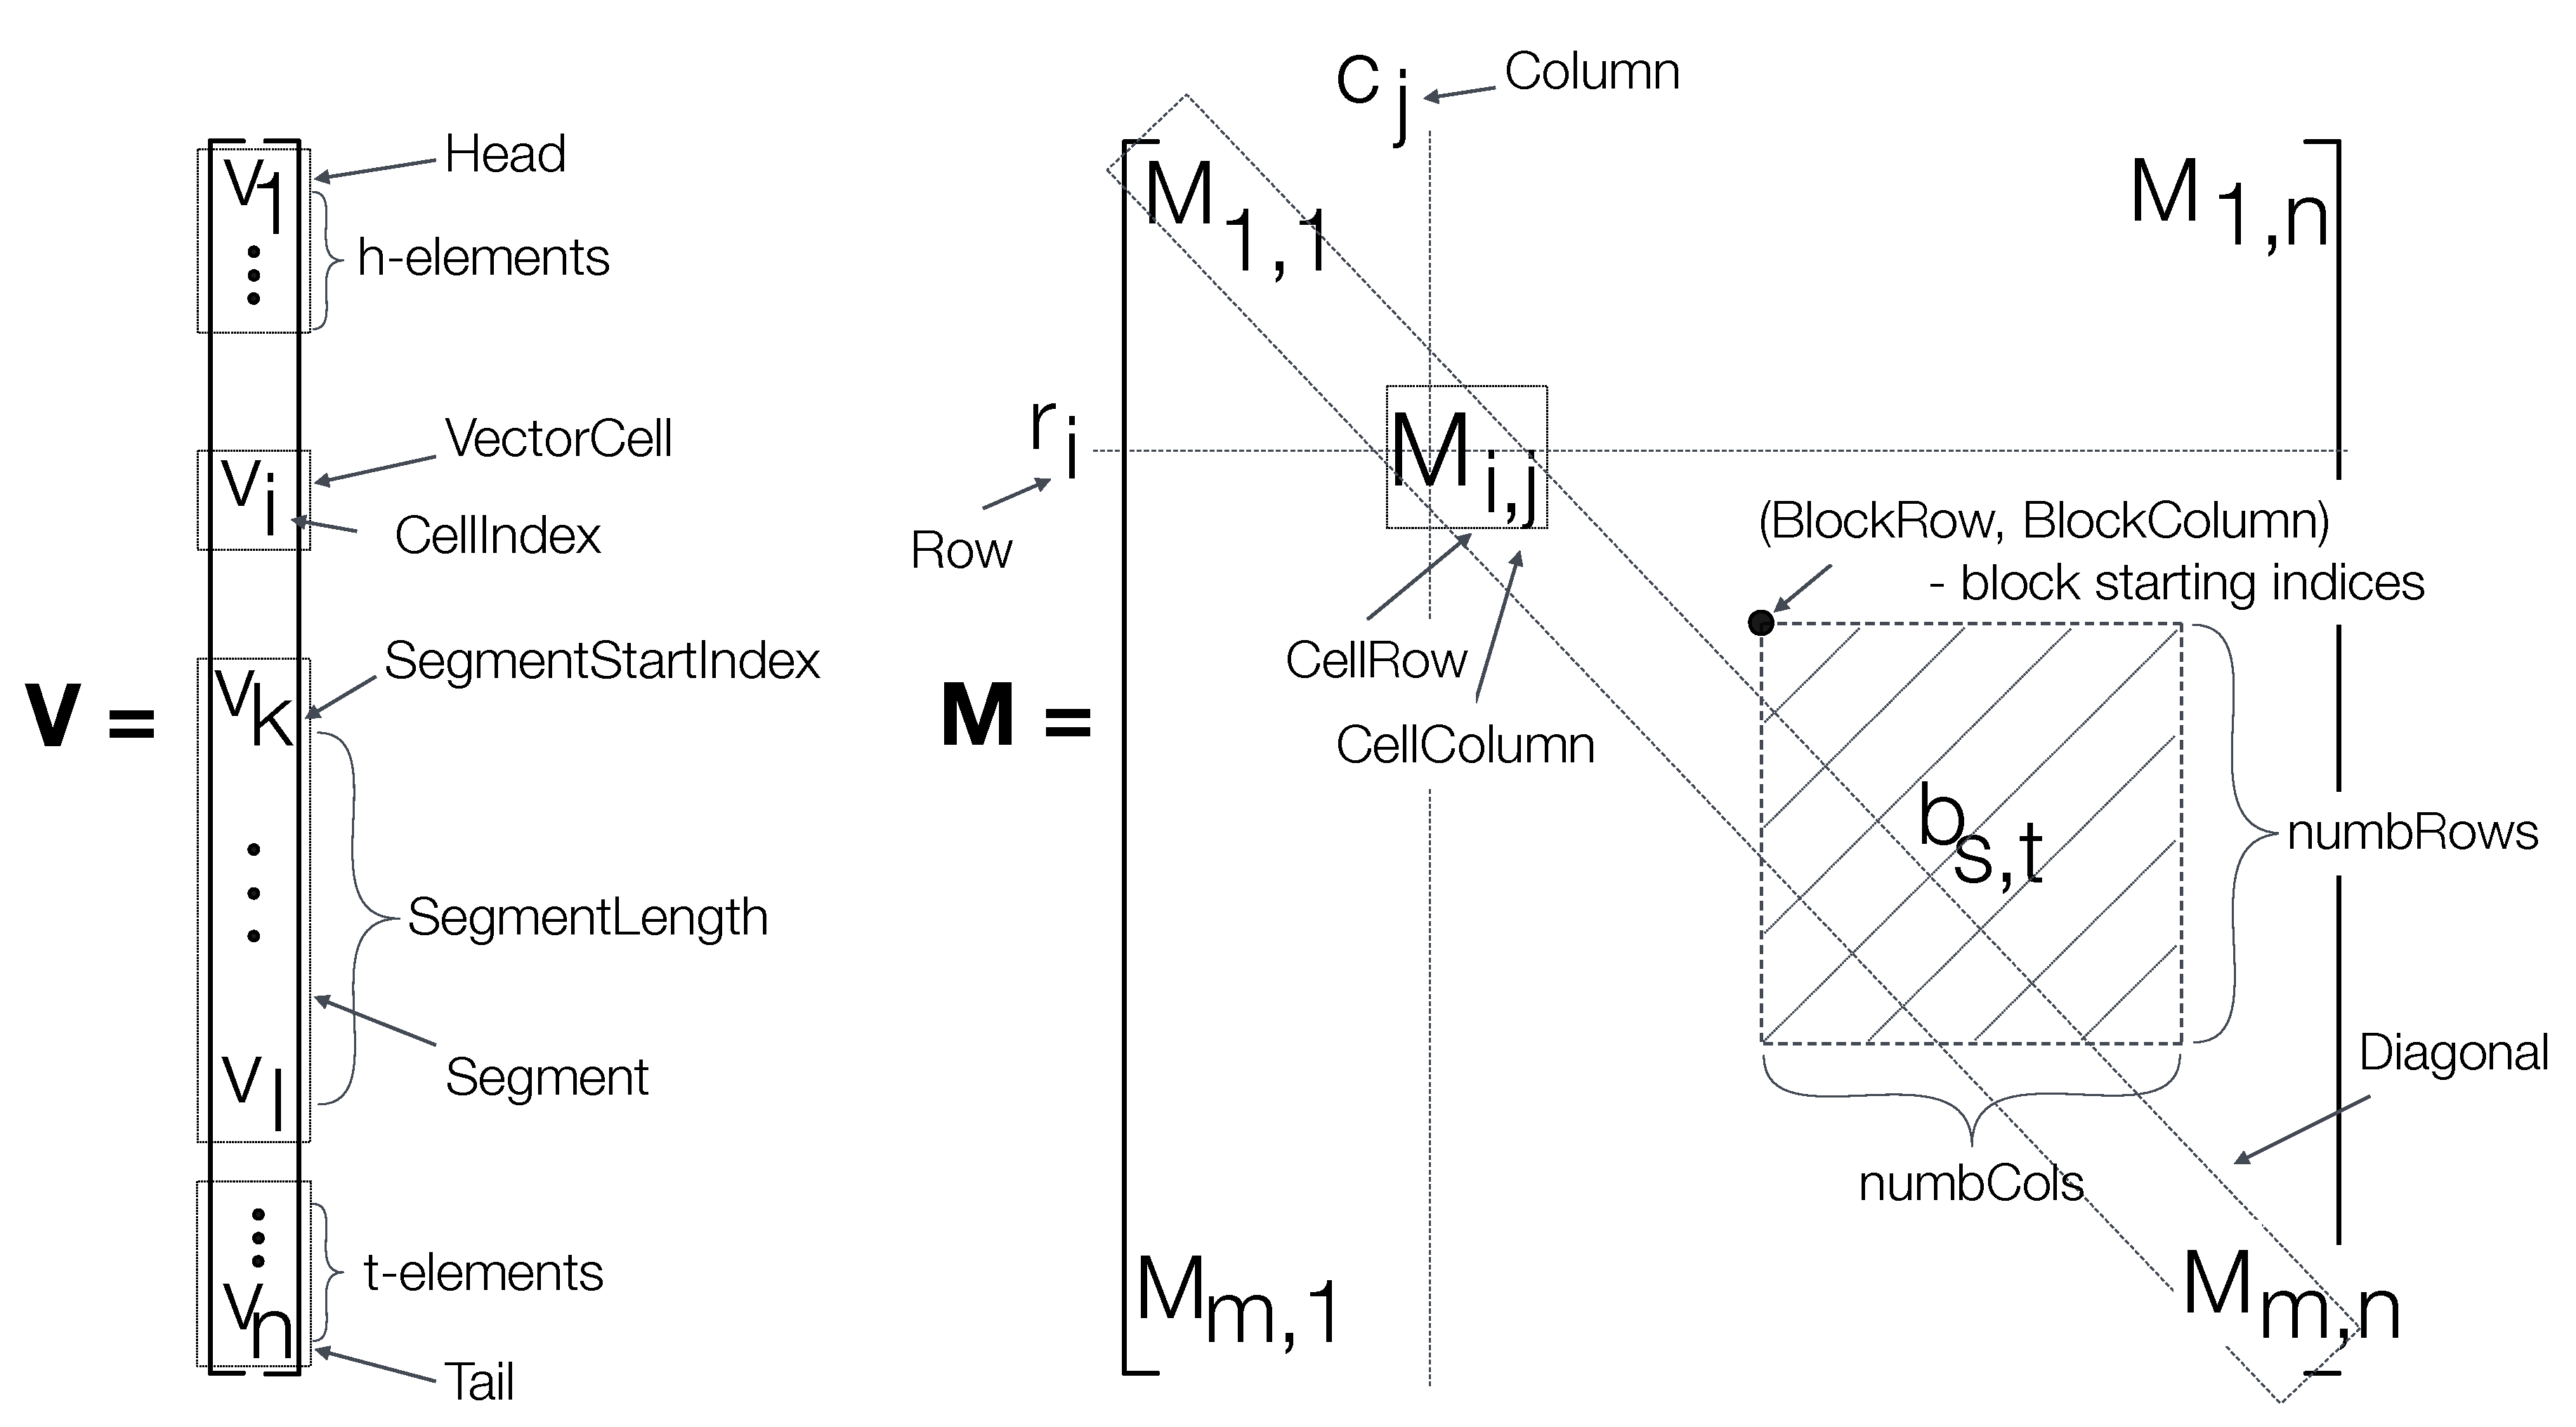
\includegraphics[width=170mm]{pics/VectorMatrixStructure}
\caption{Vector and matrix -- vocabulary and structure overview.}
\label{fig:vectorMatrix}
\end{figure}



%%%%%%%%%%%%%%%%%%%%%%%%%%%%%%%%%%%%%%%%%%%%%%%%%%%%%%%%%%%%%%%%%%%%%%
\subsection{Vector structure with examples}
\label{subsec:vectorType}
The index for vector or matrix elements start with 1. Vectors are assumed to 
be column vectors. We provide both support for populating and reading 
vectors. 

\subsubsection{Populating vectors}
The elements and attributes that are available to handle most common situation,
schematically visualised in Figure \ref{fig:vectorMatrix} (left).

Table \ref{tab:twoOptionsForVector} shows two examples of how a sparse vector 
[0,2,0,0,5,0,0,0,0,0] can be coded in \pharmml. A vector is either 
encoded explicitly with \xelem{VectorElements} using a mixture of numbers 
and symbol references or using the \xelem{VectorCell} elements (bottom right). 
The latter option, allowing to avoid unnecessary repetitions, requires the 
\xatt{default} attribute to define all remaining entires and \xatt{length} attribute 
to infer the vector length.

\begin{table}[hb!]
\setlength{\tabcolsep}{5pt}
\begin{center}
\begin{tabular}{ll}
  \hline
 Population of a vector using  	& Populating a vector using \xelem{VectorCell} \\
 \xelem{VectorElements}		& and attributes \xatt{default} and \xatt{length} \\
  \hline
\lstset{language=XML}
\begin{lstlisting}
<SimpleParameter symbId="V1">
    <ct:Assign>
        <ct:Vector length="10">
            <ct:VectorElements>
                <ct:Real>0</ct:Real>
                <ct:Real>2</ct:Real>
                <ct:Real>0</ct:Real>
                <ct:Real>0</ct:Real>
                <ct:SymbRef symbIdRef="fifthElement"/>
                <ct:Real>0</ct:Real>
                <ct:Real>0</ct:Real>
                <ct:Real>0</ct:Real>
                <ct:Real>0</ct:Real>
                <ct:Real>0</ct:Real>
            </ct:VectorElements>
        </ct:Vector>
    </ct:Assign>
</SimpleParameter>
\end{lstlisting}  
    &
    \lstset{language=XML}
    \begin{lstlisting}
<SimpleParameter symbId="V2">
    <ct:Assign>
        <ct:Vector default="0" length="10">
            <ct:VectorCell>
                <ct:CellIndex>
                    <ct:Int>2</ct:Int>
                </ct:CellIndex>
                <ct:Real>2</ct:Real>
            </ct:VectorCell>
            <ct:VectorCell>
                <ct:CellIndex>
                    <ct:Int>5</ct:Int>
                </ct:CellIndex>
                <ct:SymbRef symbIdRef="fifthElement"/>
            </ct:VectorCell>
        </ct:Vector>
    </ct:Assign>
</SimpleParameter>
    \end{lstlisting} 
    \\
    \hline
\end{tabular}
\caption{Comparison of two encoding types of the vector [0,2,0,0,5,0,0,0,0,0].
The vector is either encoded explicitly with \xelem{VectorElements} using a mixture 
of numbers and symbol references (left) or using the \xelem{VectorCell} elements (right).
In the latter case the use of attributes  \xatt{default} and \xatt{length} is required,
otherwise the dimension of the vector could not be estimated.}
\label{tab:twoOptionsForVector}
\end{center}
\end{table}


\subsubsection{Reading vectors}
Selecting elements out of a vector is very flexible and efficient. 
Once a vector is assigned, we need a mechanism for the readout of vector
elements. This is done with the \xelem{VectorSelector} element. 
Let's consider following basic assignment operation
\begin{align}
	& m = a + V2[5] \nonumber
\end{align}
i.e. adding parameter $a$ to the fifth element of vector $V2$. 
The following code shows how this is done. 

\lstset{language=XML}
\begin{lstlisting}
           <SimpleParameter symbId="m">
               <ct:Assign>
                   <math:Equation>
                       <math:Binop op="plus">
                           <ct:SymbRef symbIdRef="a"/>
                           <ct:VectorSelector>
                               <ct:SymbRef symbIdRef="V2"/>
                               <ct:Cell>
                                   <ct:Int>5</ct:Int>
                               </ct:Cell>
                           </ct:VectorSelector>
                       </math:Binop>
                   </math:Equation>
               </ct:Assign>
           </SimpleParameter>
\end{lstlisting}

Additionally to the vocabulary we used before, we have now the \xelem{Head} and \xelem{Tail} 
methods, i.e. two ways to extract the first or last $n$ elements which number can be specified
explicitly. The following child elements allow flexible access to any vector element: 
\xelem{SymbRef} identifies the vector of interest (mandatory), 
\xelem{Cell} is used to pick one element, and
\xelem{Segment} allows to select a segment of a vector.


Assume a vector V2 that has 13 elements and we want to select only those specified by the
following indexes $i=\{1:3,\;6:8,\;10,\;12:13\}.$
\lstset{language=XML}
\begin{lstlisting}
            <SimpleParameter symbId="n">
                <ct:Assign>
                    <math:Equation>
                        <ct:VectorSelector>
                            <ct:SymbRef symbIdRef="V2"/>
                            <ct:Head><ct:Int>3</ct:Int></ct:Head>
                            <ct:Segment>
                                <ct:StartIndex><ct:Int>6</ct:Int></ct:StartIndex>
                                <ct:SegmentLength><ct:Int>3</ct:Int></ct:SegmentLength>
                            </ct:Segment>
                            <ct:Cell><ct:Int>10</ct:Int></ct:Cell>
                            <ct:Tail><ct:Int>2</ct:Int></ct:Tail>
                        </ct:VectorSelector>
                    </math:Equation>
                </ct:Assign>
            </SimpleParameter>
\end{lstlisting}


%%%%%%%%%%%%%%%%%%%%%%%%%%%%%%%%%%%%%%%%%%%%%%%%%%%%%%%%%%%%%%%%%%%%%%
\subsection{Matrix structure with examples}
\label{subsec:matrixStructure}
Similarly to the vector structure there are a few alternative options to encode a matrix.
Note, that for now matrices can be used for encoding of the correlation structure between\marginpar{COMPLETE DESCRIPTION AND SECTION} 
random effect, i.e. within the \xelem{Correlation} element only. Their use will be extended to 
handle covariance matrices of multivariate distributions and other model elements in 
a future release. The index for matrix elements start with 1.

\subsubsection{Populating matrices}
\pharmml provides multiple ways to populate matrices. 
Following matrix, $\Sigma$ can be represented as a full matrix or sparse matrix. 
\label{subsec:matrixType}
\begin{align}
\Sigma = 
  \begin{bmatrix} 
  1 & \Sigma_{12} & 0 & 0 \\
  0 & 1 & \Sigma_{23} & 0 \\
  \Sigma_{31} & 0 & 1 & 0 \\
  0 & 0 & 0 & \Sigma_{44} \nonumber \end{bmatrix} 
\end{align}

\subsubsection{Implementation of $\Sigma$ as full matrix}
This is a straightforward implementation of every matrix element explicitly using
the \xelem{MatrixRow} elements, which is used to define the matrix row-by-row.  
\lstset{language=XML}
\begin{lstlisting}
            <Correlation deviationMatrixType="CovMatrix">
                <ct:VariabilityReference>
                    <ct:SymbRef symbIdRef="indiv"/>
                </ct:VariabilityReference>
                <Matrix matrixType="Any">
                    <ct:MatrixRow>
                        <ct:RowIndex><ct:Int>1</ct:Int></ct:RowIndex>
                        <ct:Real>1</ct:Real>
                        <ct:SymbRef symbIdRef="Sigma12"/>
                        <ct:Real>0</ct:Real>
                        <ct:Real>0</ct:Real>
                    </ct:MatrixRow>
                    <!-- omitted rows 2 & 3 -->
                    <ct:MatrixRow>
                        <ct:RowIndex><ct:Int>4</ct:Int></ct:RowIndex>
                        <ct:Real>0</ct:Real>
                        <ct:Real>0</ct:Real>
                        <ct:Real>0</ct:Real>
                        <ct:SymbRef symbIdRef="Sigma44"/>
                    </ct:MatrixRow>
                </Matrix>
            </Correlation> 
\end{lstlisting}
 
\subsubsection{Implementation of $\Sigma$ as sparse matrix}
Here the $\Sigma$ matrix is implemented using \xelem{MatrixCell}, which is useful for matrices with a few non-zero elements. Only four 
values have to be stored while the rest is encoded using \xatt{diagDefault} and \xatt{offDiagDefault} attributes.
\lstset{language=XML}
\begin{lstlisting}
            <Correlation deviationMatrixType="CovMatrix">
                <ct:VariabilityReference>
                    <ct:SymbRef symbIdRef="indiv"/>
                </ct:VariabilityReference>
                <Matrix matrixType="Any" diagDefault="1" offDiagDefault="0">
                    <ct:MatrixCell>
                        <ct:CellRow><ct:Int>1</ct:Int></ct:CellRow>
                        <ct:CellColumn><ct:Int>2</ct:Int></ct:CellColumn>
                        <ct:SymbRef symbIdRef="Sigma12"/>
                    </ct:MatrixCell>
                    <!-- omitted MatrixCell's in rows 2 & 3 -->
                    <ct:MatrixCell>
                        <ct:CellRow><ct:Int>4</ct:Int></ct:CellRow>
                        <ct:CellColumn><ct:Int>4</ct:Int></ct:CellColumn>
                        <ct:SymbRef symbIdRef="Sigma44"/>
                    </ct:MatrixCell>
                </Matrix>
            </Correlation>
\end{lstlisting}  
Note that the attributes \xatt{diagDefault} and \xatt{offDiagDefault}
are set to 1 or 0, respectively, which makes the matrix encoding very efficient.

\subsubsection{Example 1 -- Covariance matrix with expressions}
The elements of a matrix can contain arbitrary expressions. For example, the following covariance matrix
\begin{align}
\Sigma = 
  \begin{bmatrix} 
  	\sigma_V^2  			& \rho\; \sigma_V \sigma_k \\
        \rho\; \sigma_V \sigma_k   	& \sigma_V^2 \nonumber \\
\end{bmatrix} 
\end{align}
is easily implemented as the following code shows

\lstset{language=XML}
\begin{lstlisting}
            <Correlation deviationMatrixType="CovMatrix">
                <ct:VariabilityReference>
                    <ct:SymbRef blkIdRef="modelVar" symbIdRef="indiv"/>
                </ct:VariabilityReference>
                <Matrix matrixType="Any">
                    <ct:MatrixRow>
                        <ct:RowIndex><ct:Int>1</ct:Int></ct:RowIndex>
                        <math:Equation>
                            <math:Binop op="power">
                                <ct:SymbRef symbIdRef="sigma_V"/>
                                <ct:Real>2</ct:Real>
                            </math:Binop>
                        </math:Equation>
                        <math:Equation>
                            <math:Binop op="times">
                                <ct:SymbRef symbIdRef="rho"/>
                                <math:Binop op="times">
                                    <ct:SymbRef symbIdRef="sigma_V"/>
                                    <ct:SymbRef symbIdRef="sigma_k"/>
                                </math:Binop>
                            </math:Binop>
                        </math:Equation>
                    </ct:MatrixRow>
                    <!-- omitted 2nd row -->
                </Matrix>
            </Correlation>
\end{lstlisting}  


%%%%%%%%%%%%%%%%%%%%%%%%%%%%%%%%%%%%%%%%%%%%%%%%%%
\subsubsection{Reading matrices}
Once a matrix is assigned, we need a mechanism for the readout of its elements. 
This is done with the \xelem{MatrixSelector} element. 
Following code shows few examples of how to access single element or 
row from the $\Sigma$ matrix defined in previous example.

\lstset{language=XML}
\begin{lstlisting}
            <!-- extract one element -->
            <SimpleParameter symbId="rho_tlag_ka">
                <ct:Assign>
                    <math:Equation>
                        <ct:MatrixSelector>
                            <ct:SymbRef symbIdRef="Omega"/>
                            <ct:Cell>
                                <ct:RowIndex><ct:Int>1</ct:Int></ct:RowIndex>
                                <ct:ColumnIndex><ct:Int>2</ct:Int></ct:ColumnIndex>
                            </ct:Cell>
                        </ct:MatrixSelector>
                    </math:Equation>
                </ct:Assign>
            </SimpleParameter>
            
            <!-- extract 2nd row -->
            <ct:Variable symbolType="real" symbId="SecondRow">
                <ct:Assign>
                    <math:Equation>
                        <ct:MatrixSelector>
                            <ct:SymbRef symbIdRef="Omega"/>
                            <ct:Row>
                                <ct:Int>2</ct:Int>
                            </ct:Row>
                        </ct:MatrixSelector>
                    </math:Equation>
                </ct:Assign>
            </ct:Variable>
\end{lstlisting}


\section{Representing statistics}

As can be seen in chapter \ref{chap:mathsdefn}, \pharmml relies on the
ability to use probability distributions to describe the variability
in a pharmacometric model. Admittedly, the most commonly used
distribution is the normal distribution (or transformations of it),
but our intention is that \pharmml will have the flexibility to
describe a wide range of probability distribution types. To do this
the languages uses \uncertml version
3\footnote{\url{http://www.uncertml.org}}, which is an XML Schema
based language that aims to ``describe and exchange
uncertainty''. UncertML supports all the commonly used continuous and
discrete probability distributions and so more than adequately
supports the needs of \pharmml.  As an example we can show how the
normal distribution $\mathcal{N}(0, \omega^2)$ can be defined in
\uncertml.
% shown in listing \ref{code:normal-dist-eg}.
\lstset{language=XML}
\begin{lstlisting}
<NormalDistribution xmlns="http://www.uncertml.org/3.0"
    definition="http://www.uncertml.org/distributions/normal">
    <mean>
        <rVal>0</rVal>
    </mean>
    <stddev>
        <var varId="omega"/>
    </stddev>
</NormalDistribution>
\end{lstlisting}

% \begin{listing*}[htb]
% \inputxml{normal.xml}
% \caption{XML code encoding the normal distribution, $\mathcal{N}(0,
%   1)$.}
% \label{code:normal-dist-eg}
% \end{listing*}


% \section{Representing the Structural Model}

% In \pharmml one of our aims has been to reuse existing standards where it
% makes sense to do so. One standard that is suited for this purpose is
% \sbml. It can be used to encode systems of ODEs or algebraic
% equations, but it can also encode more complicated mechanistic models
% too. For example models that describe signalling pathways spanning
% multiple compartment. Therefore, it is our preferred mechanism for
% representing the structural model in \pharmml.

% However, in order to use a structural model encoded in \sbml we need
% to somehow incorporate it into the \pharmml document. We do this with the
% \xelem{Import} element as can be seen in listing
% \ref{code:import-eg}. In doing so the import statement maps equivalent
% variables in the \pharmml document to those in the \sbml model.

% \begin{listing*}[htb]
% \inputxml {sbml-import1.xml}
% \caption{This snippet illustrates how we map the parameters
%   and variables in the \pharmml document to the \sbml model. The model
%   itself is identified by a URL and the type of model is identified as
% \attval{sbml}. The variables and the parameters (not shown) in the
% \pharmml document are mapped to those in the \sbml model.}
% \label{code:import-eg}
% \end{listing*}

% In addition to incorporating \sbml models we can also incorporate
% other structural models defined in \pharmml. This mechanism is there for
% completeness and is not the preferred method for including models,
% so we will not go into in more detail here.

\section{Time}
\label{sec:independent-var}

Time is required by most pharmacometric models and in \pharmml it can
be referred to explicitly. The symbol used for the time variable is
configurable at the beginning of the document as shown below:

\lstset{language=XML}
\begin{lstlisting}
<PharmML xmlns="http://www.pharmml.org/pharmml/0.6/PharmML"
    xmlns:xsi="http://www.w3.org/2001/XMLSchema-instance"
    xsi:schemaLocation="http://www.pharmml.org/pharmml/0.6/PharmML ..."
    xmlns:math="http://www.pharmml.org/pharmml/0.6/Maths"
    xmlns:ct="http://www.pharmml.org/pharmml/0.6/CommonTypes"
    xmlns:ds="http://www.pharmml.org/pharmml/0.6/Dataset"
    xmlns:design="http://www.pharmml.org/pharmml/0.6/TrialDesign"
    writtenVersion="0.6">
    <ct:Name>IOV1 with covariates</ct:Name>
    <IndependentVariable symbId="t"/>
\end{lstlisting}

Rather than time we call the element \xelem{IndependentVariable}
because this is more correct and because you could define a model that
uses another quantity than time as the independent variable (e.g.\xspace
dose in a dose-response model). Note that the independent variable
always has a real type.

\section{Element identifier}
\label{sec:element-id}

To enable other resources to refer to
specific pieces of information in a \pharmml document,
every XML element in the document with an optional unique
identifier is provided. The listing below shows how the \xatt{id} attribute is
used:
%
\lstset{language=XML}
\begin{lstlisting}
<FixedEffect id="e10" symbId="beta_V">
    <Covariate>
        <ct:SymbRef  symbIdRef="W"/>
    </Covariate>
</FixedEffect>
<FixedEffect id="e13" symbIdRef="beta_Cl">
    <Covariate>
        <ct:SymbRef symbIdRef="W"/>
    </Covariate>
</FixedEffect>
<RandomVariable id="e16" symbId="eta_V">
    <ct:VariabilityReference id="e17">
        <ct:SymbRef id="e18"  blkIdRef="model" symbIdRef="level"/>
   </ct:VariabilityReference>
   <!-- Snip -->
</RandomVariable>
\end{lstlisting}
%
The \xatt{id} attribute is optional and need only be
used for elements that you want to refer to. There are no rules other
than that the identifier must be unique within the \pharmml document.
Thus to refer to a specific part of a document all you need to define is
the location of the document and the identifier. So assuming that the
above code snippet is found in a file called ``testFile.xml'' a
suitable (relative) URI that refers to the random variable in the
example might be \url{testFile.xml#e16}.

The benefit of this approach is that the \xatt{id} attribute can
easily be made available programmatically and searched on with a class
library generated from the XML Schema.
%\footnote{We considered using the XPath
% standard\cite{xpath} to identify elements using what is in effect an
% XMl query language, but we felt that it would be very difficult to
% execute such queries on a class library encode in a programming
% language the query is on the XML not attributed help within the prograsuch as
% Java, which is what you would need to do when interacting with
% \pharmml via the libPharmML API (see section
% \ref{sec:libpharmml}).
This mechanism is also used successfully by SBML \cite[Section
6]{sbmll3v1c}. You will see in the sections below (sections \ref{sec:annotation} and
\ref{sec:extension}) how we take advantage of this mechanism to
annotate and extend a \pharmml document.

\section{Ordering modelling steps}

Descriptions in a modelling step are declarative, describing what
was done, what algorithms were used and what their properties were.

\begin{figure}[htb]
 \centering
  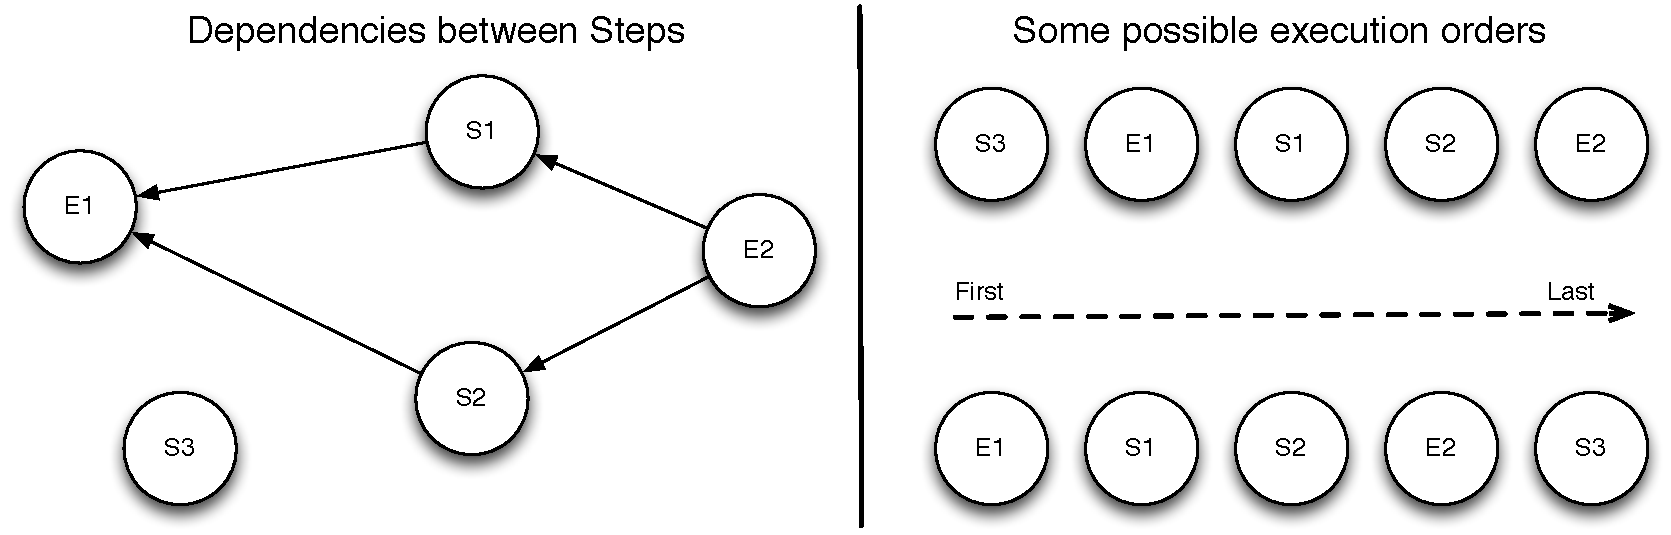
\includegraphics[width=1\linewidth]{Figures/ModellingStepDeps}
  \caption{An example of the dependencies between modelling steps is
    shown on the left. The arrow indicates the direction of the
    dependency so step S1 is dependent on the successful completion of
    step E1. So in this example step E1 must be executed before step
    S1 and S2, and those steps must both execute before step E2. On
    the right-hand figure we show two possible execution orders that
    correspond to the task dependecies on the left. It is important to
    remember that, as in this example, there can be more than one
    execution order for a given set of task dependencies.}
  \label{fig:modellingstep_deps}
\end{figure}

The \emph{Modelling Steps} section has two components that describe
simulation or estimation tasks. Multiple tasks can be linked together so
that a given estimation task can be placed before a given simulation
task or no order can be given in which case tasks can be executed in
parallel or in any order. A task is ordered by defining its dependent
tasks: tasks that must complete successfully before it can start (see
figure~\ref{fig:modellingstep_deps}). In this way the modelling steps
make no assumptions about how or where its tasks are executed, but
provides enough information for a workflow engine to parallelise the
execution of its tasks successfully, should it wish to.

At the moment tasks cannot specify how output is generated from either
an Estimation or Simulation step. A result of this restriction is that
it is \emph{not} possible to exchange information from one modelling
step to another: for example to use the output of an estimation to set
the parameter values in an estimation. We recognise that this is a
limitation of the current version and this functionality will be
provided in a future release of \pharmml.


\section{Supporting Resources}
\label{sec:supporting-res}

\subsection{Metadata: annotating the \pharmml document}
\label{sec:annotation}

As has been stated in Chapter \ref{chap:scope}, the purpose of
the \pharmml document is to provide a mathematical and structural
description of a pharmacometric model, sufficient for it to be
executed. Additional information, such as a description of the disease
process being modelled, the exact estimation algorithm or a
publication describing the model is not included in the \pharmml
document. Typically called metadata, this information is very 
important and \pharmml provides support for external annotation.

\begin{figure}[htbp]
\centering
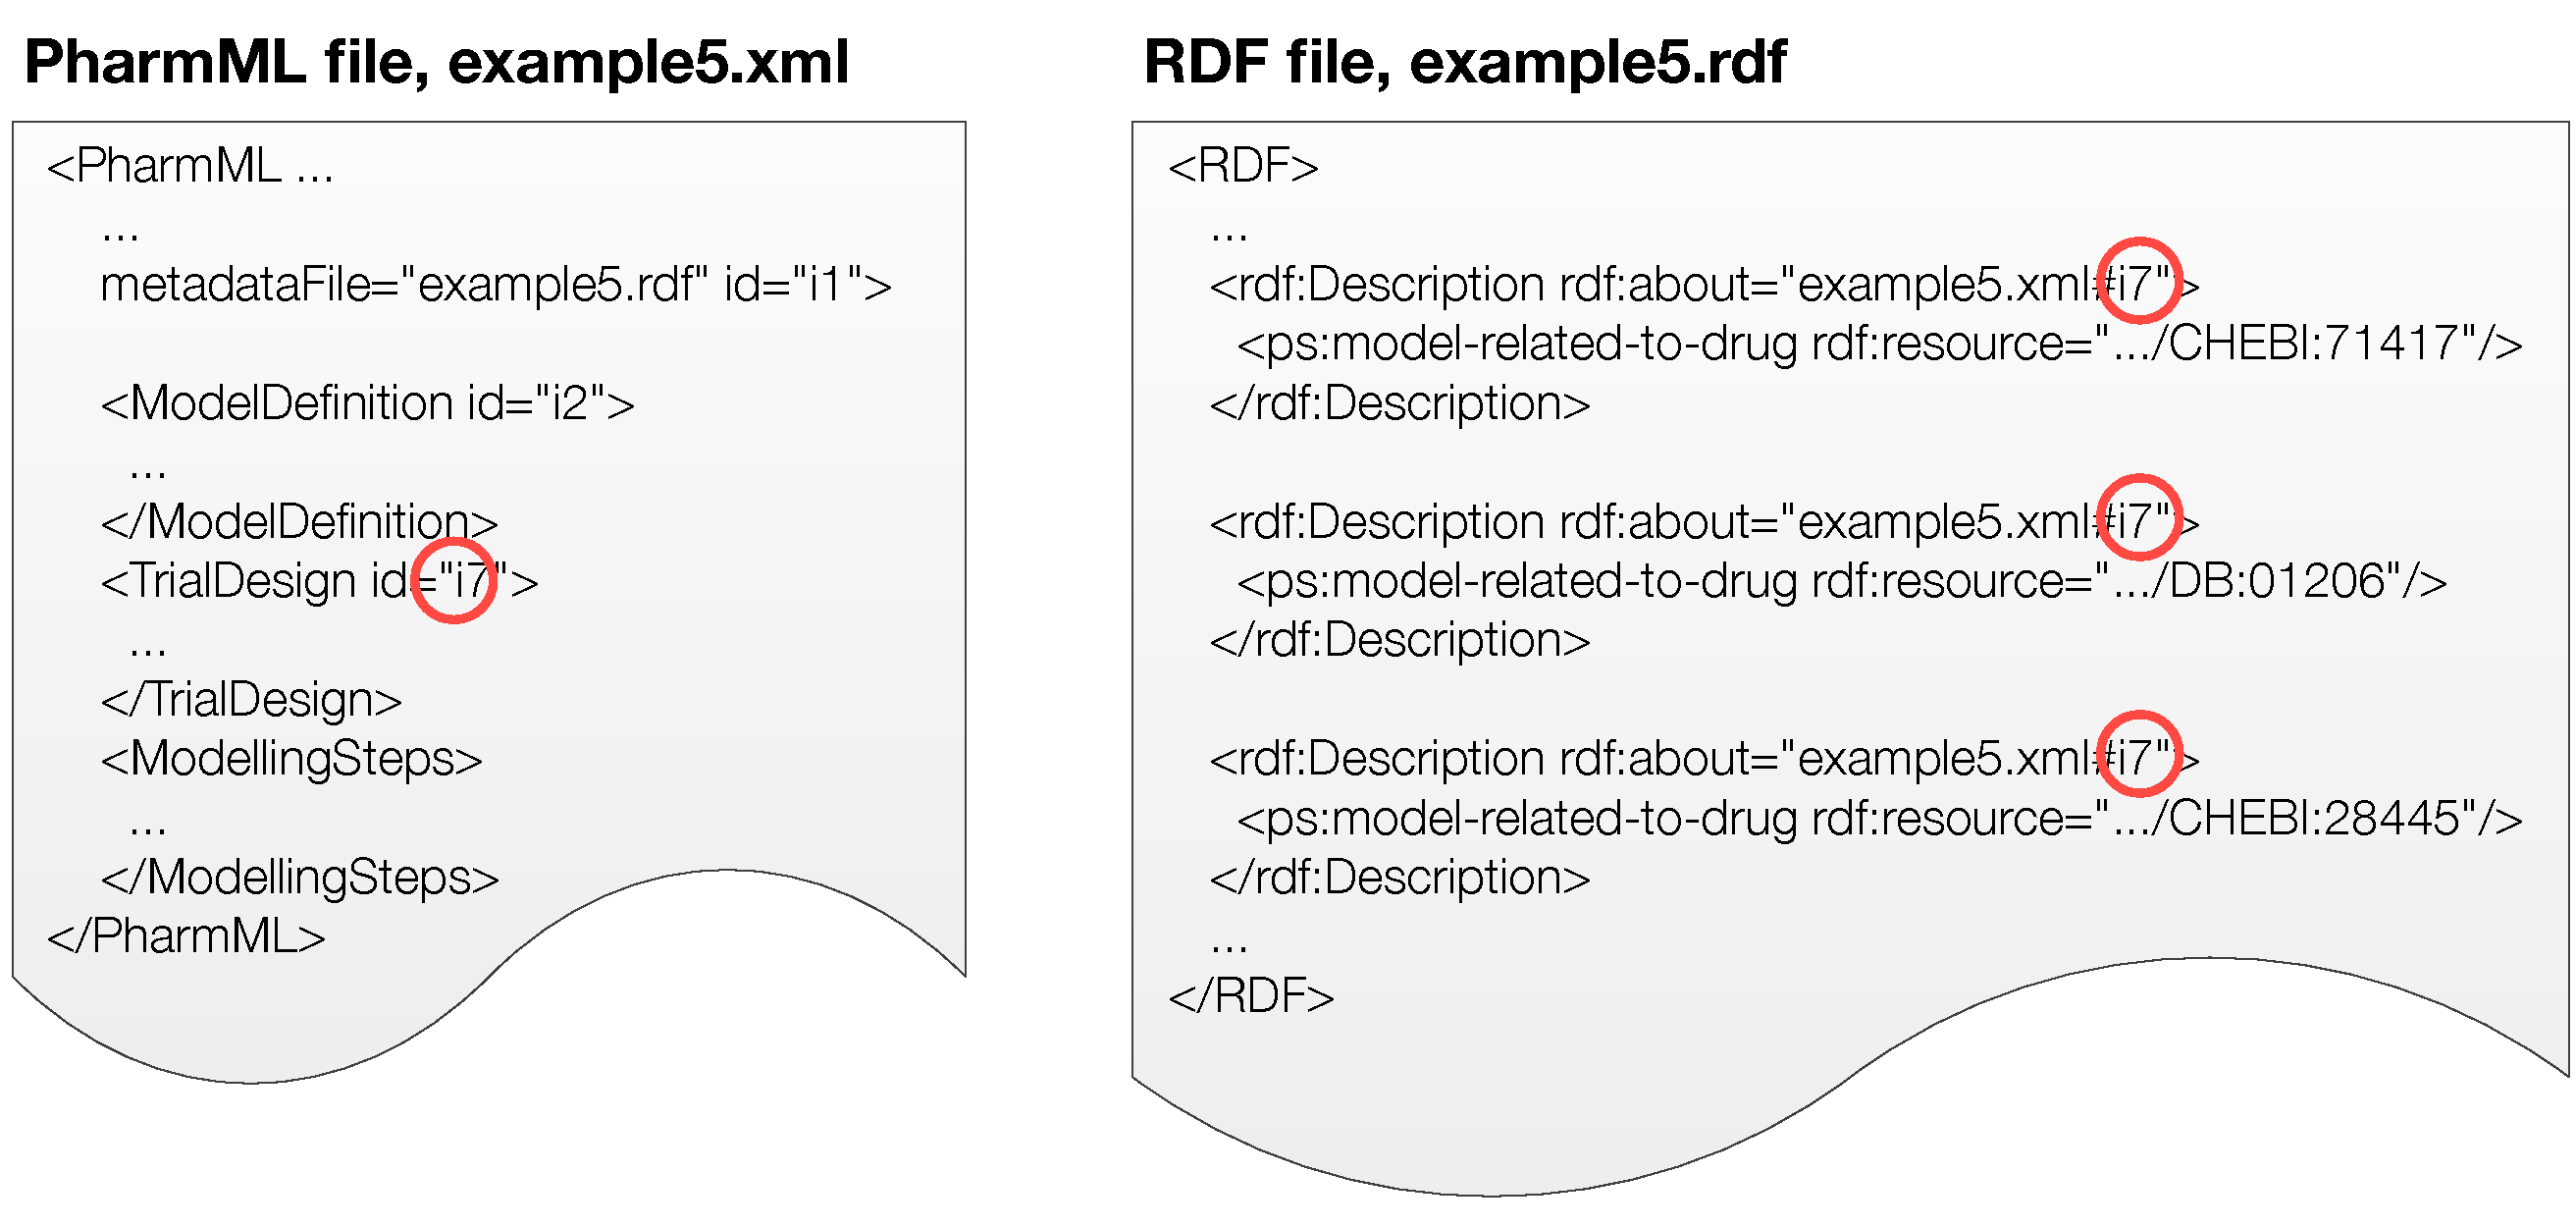
\includegraphics[width=0.8\linewidth]{pics/PharmML_RDF.pdf}
\caption{On schematic overview of the \pml, \emph{example5.xml} and RDF, 
\emph{example5.rdf}, files relationships. Note, that we use here, for the sake of clarity, 
a simplified RFD statements. See the code snippet at the end of this section 
for the correctly formatted RDF file.}
\label{fig:pharmmlRdf}
\end{figure}

We expect such metadata comes in the form of ontological annotation and
while the detail of what will be annotated is out of scope of this
document it is important to stress that every \pml element can be annotated. 
This is done by adding an attribute, e.g. \xatt{id="i7"}, to the \xelem{TrialDesign}
element, see Figure \ref{fig:pharmmlRdf}.\footnote{More information on 
annotating \pharmml models are described in the \pharmml Metadata Specification.} 
The following example gives you a flavour of what an RDF annotation of 
a \pharmml document would look like. 
The metadata above is encoded in RDF-XML\footnote{See \url{rdf-xml}}
and annotates 3 external terms; CHEBI:71417, DB01206, and CHEBI:28445.

\begin{figure}[htbp]
\centering
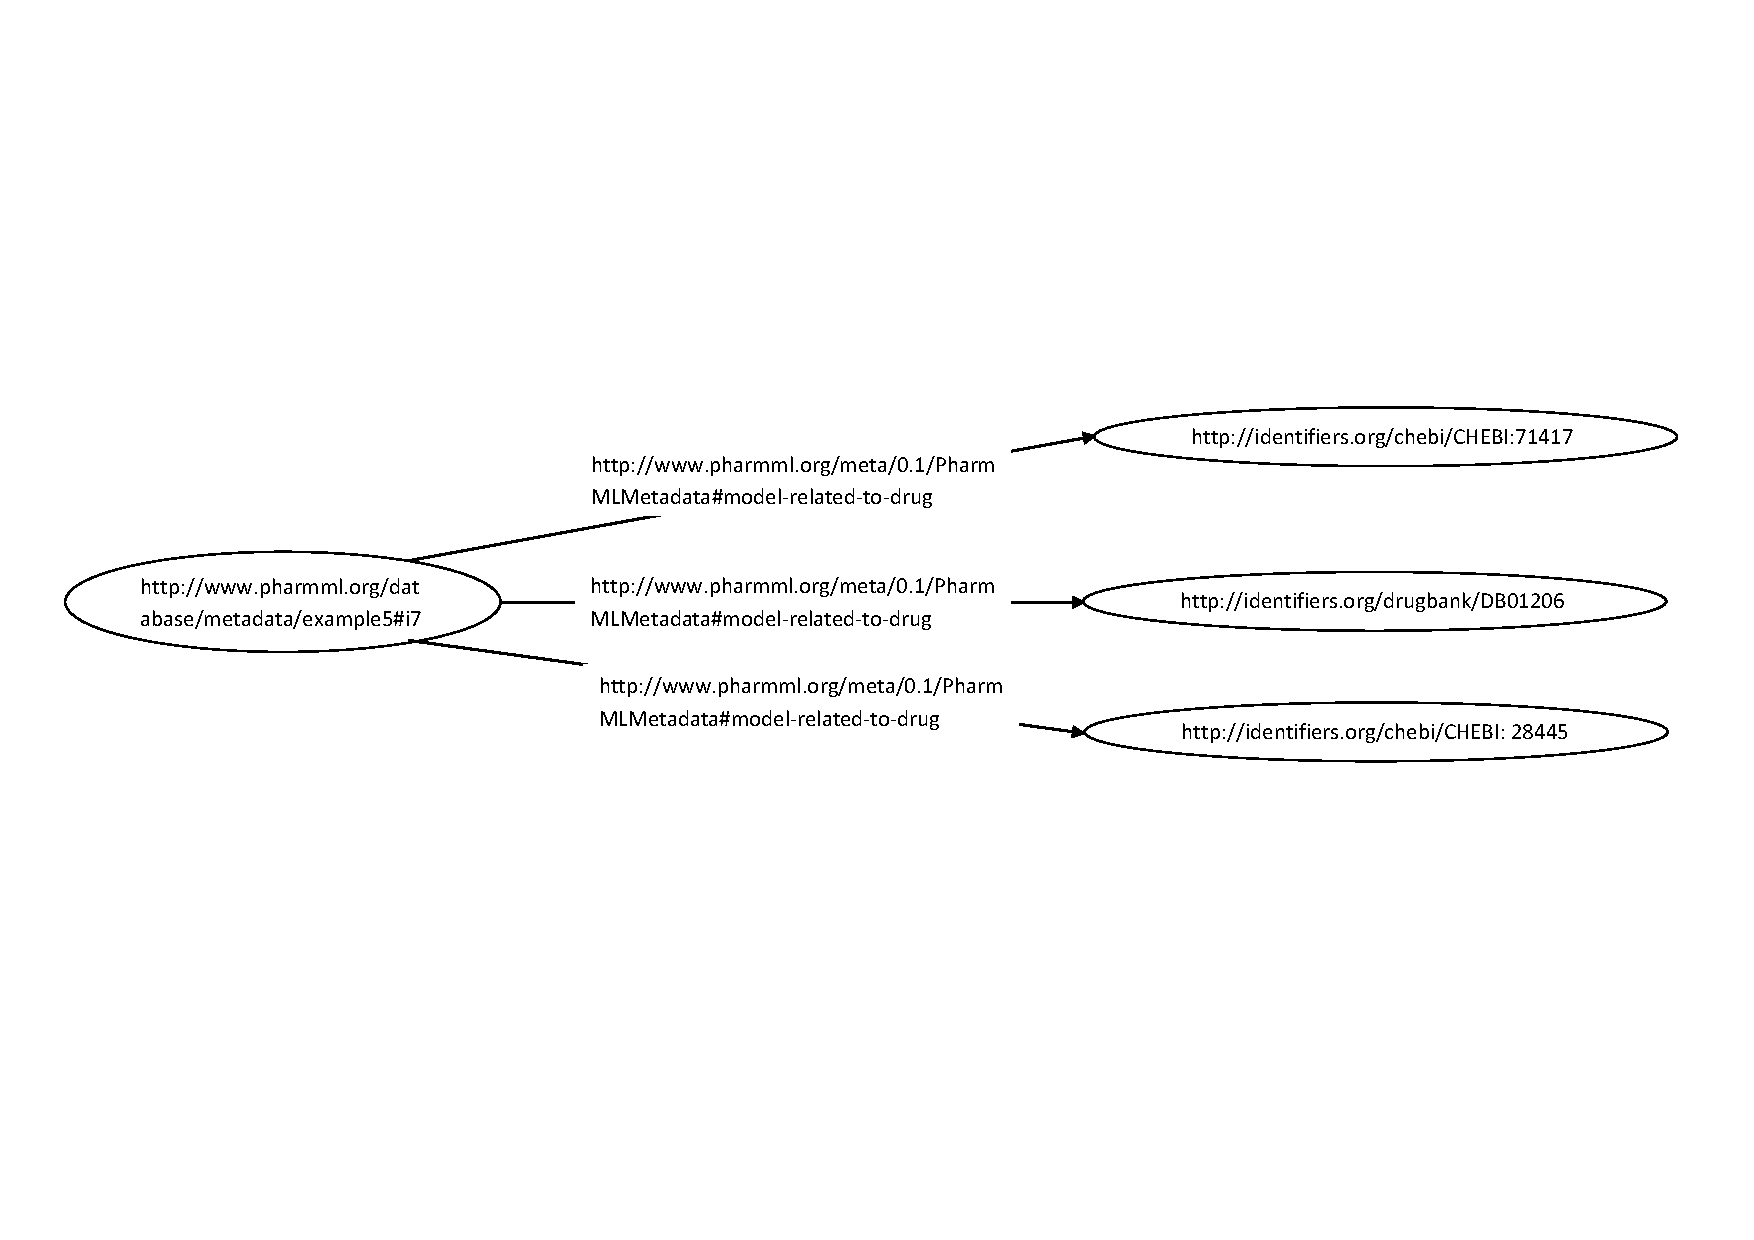
\includegraphics[width=0.95\linewidth]{pics/metadatadiagram.pdf}
\caption{This figure illustrates how information in the RDF example is
organised. Simply put the subject of the annotation is on the left and
is annotated by the object on the right. The meaning of that
annotation is described by the \emph{predicate} term labelling the
arrow. So reading the top subject from left to right we understand that
element assigned the attribute \xatt{i7} is \emph{model-related-to-drug} at \emph{CHEBI:71417}.}
\label{fig:rdf-graph}
\end{figure}
This is a basic example, but it illustrates how the \pharmml document can be annotated 
using metadata described in a separate RDF document

%
\lstset{language=XML}
\begin{lstlisting}
<rdf:RDF
    xmlns:rdf="http://www.w3.org/1999/02/22-rdf-syntax-ns#"
    xmlns:rdfs="http://www.w3.org/2000/01/rdf-schema#"
    xmlns:base="http://www.pharmml.org/database/metadata/example5#"
    xmlns:example5="http://www.pharmml.org/database/metadata/example5#"
    xmlns:ps="http://www.pharmml.org/meta/0.1/PharmMLMetadata#"> 
    
    <rdf:Description rdf:about="#i7">
        <ps:model-related-to-drug rdf:resource="http://identifiers.org/chebi/CHEBI:71417"/>
        <ps:model-related-to-drug rdf:resource="http://identifiers.org/drugbank/DB01206"/>
        <ps:model-related-to-drug rdf:resource="http://identifiers.org/chebi/CHEBI:28445"/>
    </rdf:Description>
</rdf:RDF>
\end{lstlisting}
\marginpar{CORRECT URL's}

\subsection{Extending PharmML}
\label{sec:extension}

As with any standard there will be circumstances when it does not
represent all the information that you would like and it would be
convenient to extend it. Typically there are two scenarios where this
is likely to be the case. The first is when the information is genuinely
not supported by \pharmml. This may be because it has not been
implemented yet, or it may be that there is no consensus about whether
this information should be included or no agreement about the best way
to represent it. The second scenario is when you want to
add application specific information to a \pharmml document. Perhaps
because a tool wishes to use \pharmml as its native storage format in
which case it would also want to store information about application
settings etc.

Whatever the reason \pharmml can be extended. Like the metadata
descriptions above (section \ref{sec:annotation}) this approach relies
on the element identifier (see section~\ref{sec:element-id}). The
recommended approach is that you develop a separate XML document
(typically in a separate file), which we will call the extension
document, using any XML representation you choose. Where information
in the extension document relates to the content of the \pharmml
document then you can refer to the relevant XML element using its
identifier.

\begin{figure}[htb]
\centering
  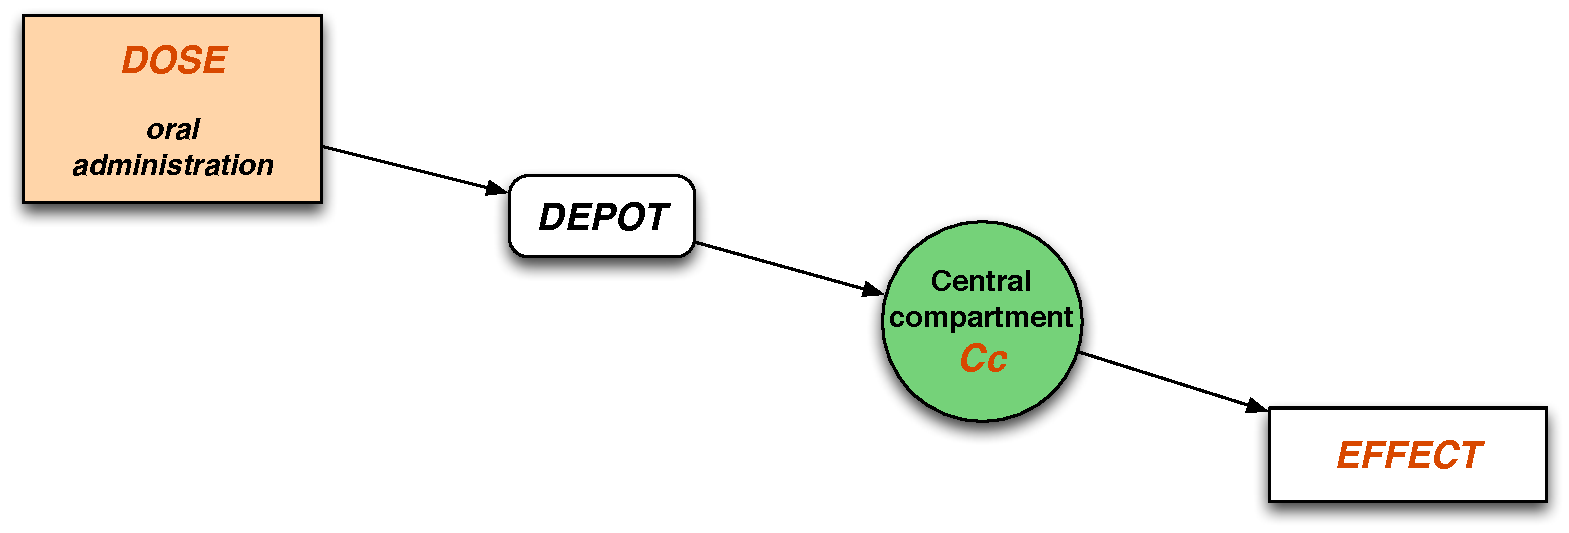
\includegraphics[height=0.2\textheight]{Figures/GraphicalModel}
  \caption{This diagram is reproduced from an example in the Monolix
    user manual \cite{Monolix4.1.4UserGuide:2012} and it provides a
    graphical description of a structural model. In the hypothetical
    example in the text we illustrate how you might extend \pharmml to
    link this graphic with the components of the model it represents.}
\label{fig:graphical-model}
\end{figure}

We can illustrate with an example based on the second scenario we
described above: application specific extensions. In this scenario our
software tool provides a graphical interface that lets you create a
pharmacometric model by drawing and connecting shapes such as the
diagram in figure~\ref{fig:graphical-model}. When you save the diagram
the application saves both the \pharmml that encodes the model and an
extension document that describes the graphical layout and maps the
graphical elements to the relevant parts of the model. The extension
document could look like this:
%
\lstset{language=XML}
\begin{lstlisting}
<Diagram resource="file:///anotherPharmMLFile.xml">
    <Rectangle id="1">
        <Name>Dose</Name>
        <Bounds x="10" y="10" w="50" h="30"/>
        <!-- Omitted other information such as colour and other text-->
        <Ref idRef="e35"/>
    </Rectangle>
    <!-- Omitted -->
    <Circle id="3">
        <Name>Central</Name>
        <Bounds x="10" y="200" w="45" h="45"/>
        <!-- Omitted other information such as colour and other text-->
        <Ref idRef="e46"/>
    </Circle>
    <!-- Omitted other shape definitions-->
    <Link src="1" tgt="2"/>
    <Link src="2" tgt="3"/>
    <Link src="3" tgt="4"/>
</Diagram>
\end{lstlisting}
%
The XML describes the shapes of the nodes, their location and the
connections between them. What allows it to extend the \pharmml document?
First the \xatt{resource} attribute provides a URL describing
the location of the \pharmml document being extended. Next the
\xelem{Ref} element defines a reference that points to an element in
the \pharmml document. From this information the application is able
to read both the \pharmml and the extension documents and then relate
the diagram to the relevant part of the model.

Note that while this is a hypothetical example for \pharmml, this type
of solution has been implemented by a graphical Systems Biology editor
called CellDesigner\footnote{\url{http://www.celldesigner.org}}. It uses SBML
as its native application format: encoding the model in SBML and using
SBML's extension facilities to store graphical information and other
application specific properties.

One final clarification. The extension mechanism does not require an
application to use the same XML elements as described in the example
above. The XML content of the extension document is entirely the
concern of the application. In order to extend a \pharmml document
all it must do is:
\begin{enumerate}
\item Specify how to find the \pharmml document. Using a URI is a good
  way to do this.
\item Use the element identifier to refer to the content of the \pharmml document.
\end{enumerate}

\subsection{Organising \pharmml resources}
\label{sec:pharmml-archive}

We expect that \pharmml will in normal usage consist of more than one
file. From the discussion about annotating
(section~\ref{sec:annotation}) and extending
(section~\ref{sec:extension}) \pharmml it is clear that both of these
cases require the creation of resources that are closely
related to a \pharmml document. It is therefore desirable that they
are kept together and exchanged and used together.

\begin{figure}[htb]
\centering
  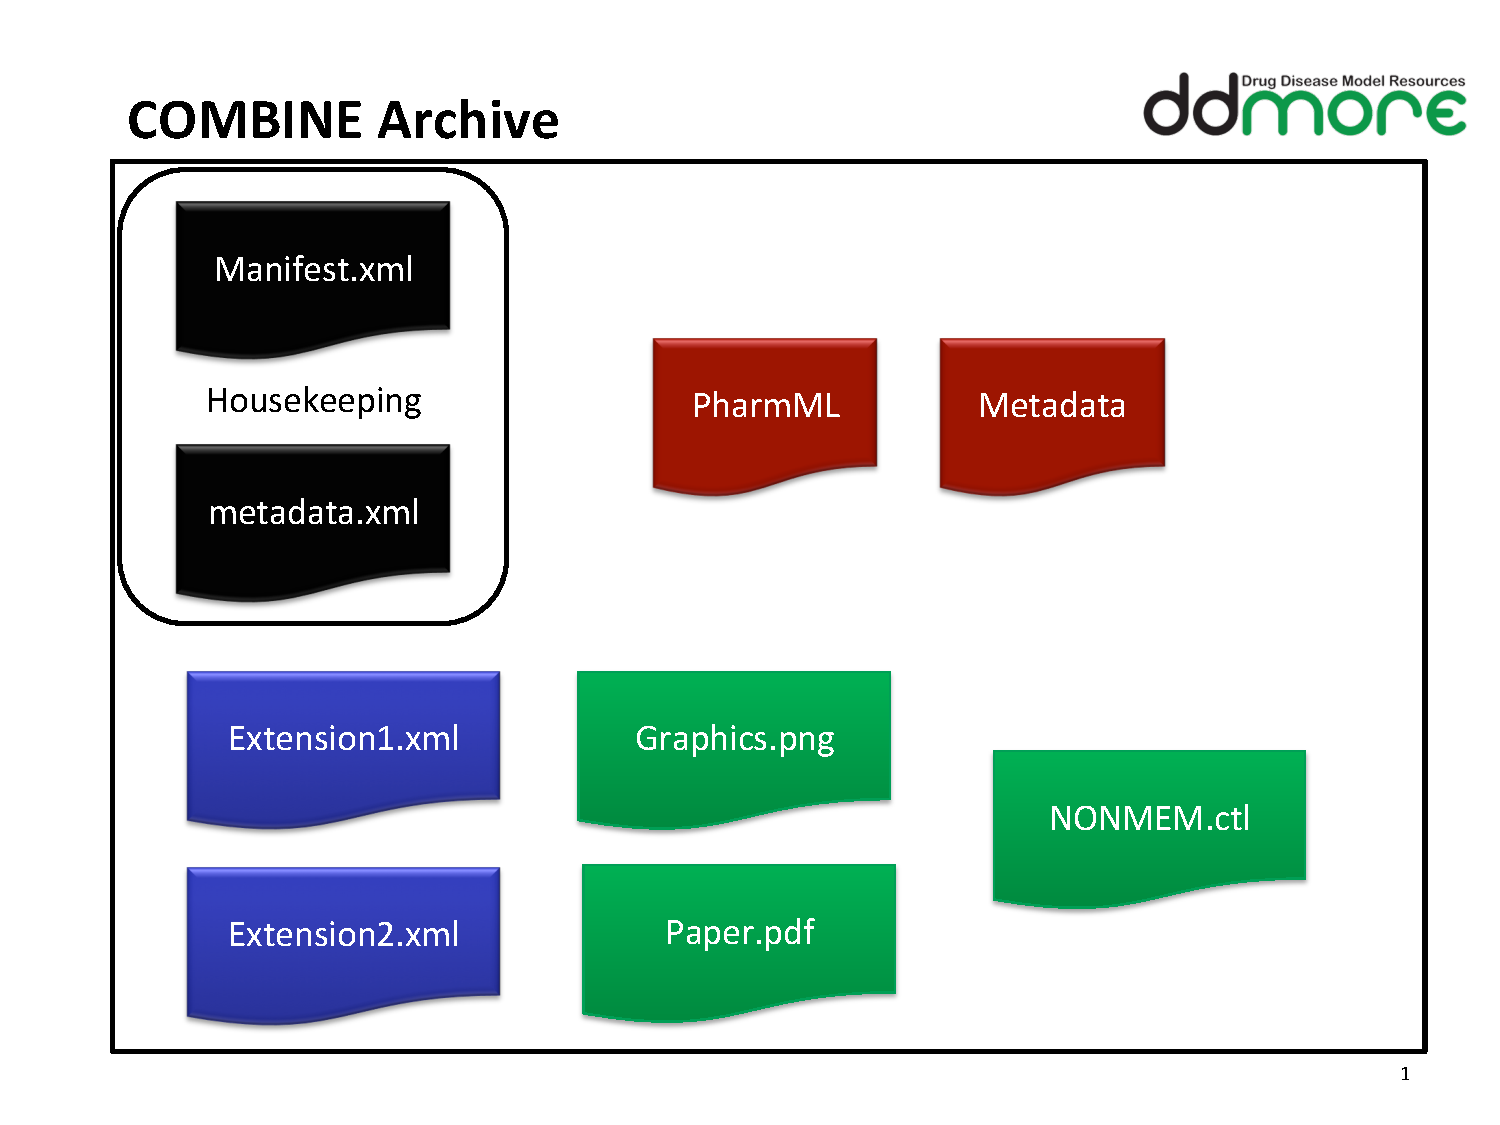
\includegraphics[width=0.6\textwidth]{Figures/AchiveOverview}
  \caption{An overview of how a COMBINE archive may be used to hold
    XML documents and files associated with a model encoded in
    \pharmml. In this example the archive holds the model and its
    metadata (in red) and two application specific extension
    documents (in blue). This also shows another advantage of using
    the archive: you can store other useful information, such as the
    original model file, relevant papers or images (in
    green). Finally, the archive contains a metadata file (in black)
    that helps an application reading the archive make sense of what
    it contains.}
  \label{fig:moml-archive-overview}
\end{figure}

An archive file can provide this functionality. It acts as a
container, and since it is a file can be easily exchanged and
stored. We recommend that you use an archive based on the emerging
COMBINE Archive
standard\footnote{\url{http://co.mbine.org/documents/archive}}. It is
based on a zip archive and holds additional information that allows
you to identify the modelling resources in the file. The exact details
of how it works is outside the scope of this document, but the
components of the archive and how it can be used to hold \pharmml
related resources is illustrated in
figure~\ref{fig:moml-archive-overview}
%\footnote{An example of a
%  CombineArchive file that contains a metadata file annotating a
%  \pharmml document can be found in \texttt{examples/CombineArchive/archive.zip}.}.

\subsection{Software support for \pharmml}
\label{sec:libpharmml}

\pharmml is a complex language. It is designed using an industry
standard, XML Schema\footnote{\url{http://www.w3.org/XML/Schema}}, which gives us the
ability to use widely available software packages to verify that the
XML file is correctly written and that elements are put in the right
place (syntax checking). However, \pharmml describes a pharmacometric
model and so there is a lot of information that is very specific to
this domain and cannot be validated by standard tools.  That's why we need
\pharmml specific software tools and libraries. Without such software
the burden of validation falls on the modelling tools reading and
writing \pharmml. Given the complexity of \pharmml's validation rules
it is unlikely that such validation would be complete and implemented
consistently, which makes our goal of exchange between modelling
tools less likely to succeed.

Therefore in parallel to the development of this specification a
software library called libPharmML\footnote{For more information see
  the libPharmML specification in the DDMoRe Interface Europe
  document repository: WP2 deliverables: \emph{D2.2
    libPharmMLTechSpec}.}\marginpar{CORRECT URL} is being developed to support it.  This will
allow you do the following:
%
\begin{enumerate}
\item Create a new \pharmml document.
\item Read an existing \pharmml document from a file (or other
  resource).
\item Write a \pharmml document to a file (or resource).
\item Validate that a \pharmml document complies with the XML Schema
  definition and the rules set out in this specification.
\end{enumerate}
%
The library is implemented in Java. There are no plans to implement an equivalent
version in another programming language, such as C++, but this could be done if
there was sufficient demand for it and sufficient developer resources were available
to implement it.
